\chapter{Smart computation of \texorpdfstring{$x^n$}{Powers}}
\label{chapter-powers}
\section{Introduction}

Nothing looks simpler than writing a function for computing $x^n$.
But on the contrary, this simple programming exercise allows us to address
advanced programming techniques such as:
\begin{itemize}
\item monadic programming, and continuation passing style
\item type classes, and generalized rewriting
\item proof engineering, in particular proof reuse
\item proof by reflection
\item polymorphism and parametricity
\item composition of correct programs, etc.
\end{itemize}



\section{Some basic implementations}
\label{sect:linear-naive}
Let us start with a very naive way of computing the $n$-th power of $x$, where
$n$ is a natural number and $x$ belongs to some type for which a multiplication and an identity element are defined.


\emph{From Module 
\href{../theories/html/additions.FirstSteps.html}{\texttt{additions.FirstSteps}}}
\label{sect: power-definitions}

\inputsnippets{FirstSteps/Defs}

An application of this function for  computing $x^n$ needs $n$ multiplications.
 Despite this lack of efficiency, and thanks to its simplicity, we keep it as a specification for more efficient and complex exponentiation algorithms.
A function will be considered a \emph{correct} exponentiation function if we can prove it is extensionally equivalent to \texttt{power}.

% \subsection{A semi-naive algorithm}

% In versions up to \texttt{V8.9.1}, the exponentiation function on type \texttt{Z} was defined as follows,
% (in modules \texttt{Coq.PArith.BinPosDef.Pos} and \texttt{Coq.ZArith.BinIntDef.Z}.

% \begin{Coqsrc}
% (** ** Iteration of a function over a positive number *)

% Definition iter {A} (f:A -> A) : A -> positive -> A :=
%   fix iter_fix x n := match n with
%     | xH => f x
%     | xO n' => iter_fix (iter_fix x n') n'
%     | xI n' => f (iter_fix (iter_fix x n') n')
%   end.

% Definition pow (x:positive) := iter (mul x) 1.
% \end{Coqsrc}


% \begin{Coqsrc}
% Definition pow_pos (z:Z) := Pos.iter (mul z) 1.

% Definition pow x y :=
%   match y with
%     | pos p => pow_pos x p
%     | 0 => 1
%     | neg _ => 0
%   end.

% Infix "^" := pow : Z_scope.
% \end{Coqsrc}

% At first sight, the function \texttt{Pos.pow} seems to be logarithmic because of the recursive structure of the help function \texttt{iter\_fix}. Unfortunately, it is obvious that a call to 
% \texttt{iter f x n} will apply $n$ times the function $f$. Thus, these exponentiation functions with binary exponents are in fact linear!

% \label{sect:slow-computation}

% \begin{Coqsrc}
% Time Compute (1 ^ 56666667)%N.
% \end{Coqsrc}

% \begin{Coqanswer}
% Finished transaction in 3.604 secs (3.587u,0.007s)   
% \end{Coqanswer}


\subsection{A logarithmic exponentiation  function}

Using the following equations, we can easily define a polymorphic exponentiation whose application requires only a logarithmic number of multiplications. 

\begin{align}
x^1 &= x \label{binary-eq1}\\
x^{2p} &= (x^2)^p \label{binary-eq2}\\
x^{2p+1} &= (x^2)^p \times x \label{binary-eq3}\\
x^1 \times a &= x \times a \label{binary-eq4}\\
x^{2p} \times a  &= (x^2)^p \times a\label{binary-eq5}\\
x^{2p+1} \times a  &= (x^2)^p \times (a\times x)\label{binary-eq6}
\end{align}


In equalities \ref{binary-eq4} to \ref{binary-eq6}, the variable $a$ plays the role
of an \emph{accumulator} whose initial value (set by \ref{binary-eq3}) is $x$.
This accumulator helps us to get a tail-recursive implementation.

For instance, the computation of $2^{14}$ can be decomposed as follows:
\begin{align*}
2^{14} &= 4^{7} \\
      &= 16^3 \times 4 \\
      &= 256^1 \times (4 \times 16) \\
      &= 16384  
\end{align*}

With the same notations as in Sect~\vref{sect:linear-naive}, we can implement this algorithm in \gallina. The following definitions are still within the scope of the 
section open in~\vref{sect: power-definitions}.



\label{polymorhic-binary_exp}

%%% ICI (presenter la fonction binaire de First_Steps )
%%%  Reprendre des explications placees ci-dessous

\vspace{4pt}

\emph{From Module
\href{../theories/html/additions.FirstSteps.html}{additions.FirstSteps}}

\inputsnippets{FirstSteps/bpowDef}
Let us  close the section \texttt{Definitions} and mark the argument \texttt{A} as implicit.
\inputsnippets{FirstSteps/EndDefs}

\begin{remark}
Our function \texttt{Pos\_bpow} can be considered as a tail recursive variant
of the following function defined in \texttt{Coq.PArith.BinPosDef}.



\begin{Coqsrc}
Definition iter_op {A}(op:A->A->A) :=
  fix iter (p:positive)(a:A) : A :=
  match p with
    | 1 => a
    | p~0 => iter p (op a a)
    | p~1 => op a (iter p (op a a))
  end.
\end{Coqsrc}

This scheme is used in \texttt{Coq.ZArith.Zpow\_alt} in order to define a logarithmic exponentiation \texttt{Zpower\_alt} on \texttt{Z} (notation : $x\,\texttt{\^{}\^{}}\,p$).

\end{remark}

\paragraph*{Remark}
Note that closing the section \texttt{Definitions} makes us lose the
handy notations \texttt{\_ * \_} and \texttt{one}. Fortunately, \emph{operational type classes} will help us to define nice infix notations for polymorphic functions (Sect.~\vref{op-classes}).

\subsection{Examples of computation}
It is now possible to test our functions with various interpretations of
$\times$ and $1$:

\inputsnippets{FirstSteps/PowerCompute}

% \subsubsection{Exponentiation on $2\times 2$ matrices}
% \label{naive-matrix}
% Our second example is a definition of $M^n$ where $M$ is a $2\times 2$ matrix
% over any ``scalar''  type $A$, assuming one can provide $A$ with a semi-ring structure~\cite{Coq}.


% %\subsubsection{Representation of $2\times 2$ matrices}

% A $2\times 2$ matrix will be simply represented by a structure with four fields;
% each field \texttt{c$ij$} is associated with the $i$-th line and $j$-th column of the considered matrix.



%\subsubsection{Matrix Multiplication}



\subsection{Computing Fibonacci numbers}

The sequence of Fibonacci numbers is defined by the following equations:

\begin{align}
F_0 & = 1 \\
F_1 & = 1 \\
F_n & = F_{n-1} + F_{n-2} \quad (n \geq 2)
\end{align}


In \coq{}, one can define this function by simple recursion.

\emph{From Library
\href{../theories/html/additions.Fib2.html}{additions.Fib2}}

\inputsnippets{Fib2/FibDef}

In~\cite{BC04}, several exercises~\footnote{Exercises 9.8 (page 270), 9.10 (page 271), 9.15 (page 276), 9.17 (page 284), and 15.8 (page 418).}
present ways to compute Fibonacci numbers, with the less number of recursive calls  as possible. Please note that these optimizations and the formal proof of their correctness are \emph{ad-hoc}, \emph{i.e.}, exclusively written for the
Fibonacci numbers.
In contrast, the optimizations we present in this document apply, in their vast majority, \emph{generic} techniques of efficient computation of powers in a monoid. 
This example of Fibonacci numbers has been developed with Yves Bertot, who wrote a first version with \texttt{SSreflect/Mathcomp}~\cite{MCB}.


\subsubsection{Using 2x2 integer matrices}
\index{maths}{Fibonacci numbers!Matrix exponentiation} 

The following properties are well known. They are left as an exercise, since they are not part of our development. 

\index{additions}{Exercises}

\begin{exercise}
  \label{exercise:fibmat}
  \begin{enumerate}
  \item 

Prove in \coq{} the following equality (for any $n\geq 2$). \label{fibmat-eq1}

\[
\left(
  \begin{array}{cc}
    1 & 1 \\
    1 & 0 
  \end{array}
\right)
\left(
  \begin{array}{cc}
    F_{n}& F_{n-1} \\
    F_{n-1} & F_{n-2}
  \end{array}
\right)
=
\left(
  \begin{array}{cc}
    F_{n+1}& F_{n} \\
    F_{n} & F_{n-1} 
  \end{array}
\right)
\]
  
\item Infer (still in \coq{}) the following equality (still for $n\geq 2$).



\[
\left(
  \begin{array}{cc}
    F_{n}& F_{n-1} \\
    F_{n-1} & F_{n-2} 
  \end{array}
\right)
= 
\left(
  \begin{array}{cc}
    1 & 1 \\
    1 & 0 
  \end{array}
\right)^n
\]

\item Write a function using the previous equality for computing the $n$-th Fibonacci number, and prove its equivalence with \texttt{fib}.

\end{enumerate}
\end{exercise}

\subsubsection{Removing duplicate computations}
\label{sect:fibonacci-mul2}


Yves Bertot's optimization relies on the observation that all the powers of
\(  \left(
  \begin{array}{cc}
    1 & 1 \\
    1 & 0 
  \end{array}
\right) \) have the form 
\(  \left(
  \begin{array}{cc}
    a+b  & a \\
    a & b
  \end{array}
\right) \) where $a$ and $b$ are natural numbers.

Thus, it is possible to remove duplicate data and computations by reflecting matrix multiplication and identity into $\mathbb{N}\times\mathbb{N}$.

If we pose $\varphi(a,b) =\left(
  \begin{array}{cc}
    a+b  & a \\
    a & b
  \end{array}
\right)$, then $\varphi(a,b)\times \varphi(c,d)=\varphi(ac + ad + bc, ac + bd)$, and
$\varphi(0,1)=  \left(
  \begin{array}{cc}
    1 & 0 \\
    0 & 1 
  \end{array}
\right) $.

\index{additions}{Exercises}
\begin{exercise}
  Prove formally these properties. \emph{Please note that their proof is not needed in our development, they just help to understand the following optimization.}
\end{exercise}


So, let us define a binary operation, which makes $\mathbb{N}\times\mathbb{N}$ a monoid (with $(0,1)$ as neutral element).


\emph{From Library
\href{../theories/html/additions.Fib2.html}{additions.Fib2}} 

\emph{The \texttt{Monoid} type class is defined 
page~\pageref{sect:monoid-def}.}

\inputsnippets{Fib2/mul2Def}
\inputsnippets{Fib2/mul2Monoid}


The following lemma is a simplification of the equality of Exercise~\ref{exercise:fibmat}.

\inputsnippets{Fib2/nextFib}

Let us consider a new definition of the Fibonacci function.

\inputsnippets{Fib2/fibMul2Def}
\inputsnippets{Fib2/fibMul2OK0}
\inputsnippets{Fib2/fibMul2OK}
\inputsnippets{Fib2/TimeFibMul2}


Thus, any function able to compute more or less efficiently powers in a monoid will
give an algorithm for computing Fibonacci numbers. Unlike the \emph{ad-hoc} aforementioned proofs of~\cite{BC04}, the correctness of such an algorithm is a direct consequence
of the correctness of the used powering function.
Several examples will be presented in the rest of this document
(in Section~\vref{sect:fibonacci-pos-bpow}).




% \begin{Coqsrc}

% Import M2.

% Arguments M2_mult {A} plus mult  _  _.
% Arguments mat {A} _ _ _ _.
% Arguments Id2 {A}  _ _.

% Definition fibonacci (n:N) :=
%  c00 N  (N_bpow  (M2_mult Nplus Nmult) 
%                  (Id2  0%N 1%N)
%                  (mat  1 1 1 0)%N 
%                  n).

% Compute fibonacci 20.
% \end{Coqsrc}

% \begin{Coqanswer}
% = 10946%N
%      : N  
% \end{Coqanswer}

\begin{todo}
Document the files contributed by Yves
\begin{itemize}
\item additions/fib.v (to rename ?)
\item additions/stub.ml (to keep inside theories/ or move to src/ ?)
\item theories/additions/make\_fib\_tests.txt (to put in a Makefile?)
\end{itemize}
\end{todo}




% \subsubsection{Remark}
% \label{sect:faster}

% Our function \texttt{N\_bpow} is really logarithmic. Let us make a comparative 
% test with Standard Library's exponentiation function on type \texttt{N} (see section~\vref{sect:slow-computation}).

% \begin{Coqsrc}
% Time Compute (N_bpow N.mul 1 1 56666667)%N.  
% \end{Coqsrc}

% \begin{Coqanswer}
% Finished transaction in 0. secs (0.u,0.s) (successful)  
% \end{Coqanswer}




\subsection{Formal specification of an exponentiation function: a first attempt}

Let us compare the functions \texttt{power} and \texttt{N\_bpow}.
The first one is obviously correct, since it is a straightforward translation of the mathematical definition.
The second one is much more efficient, but it is not obvious  that its 18-line long definition is bug-free.
Thus, we must prove that the two functions are extensionally equal (taking into account conversions
between \texttt{N} and \texttt{nat}).

More abstractly, we can define a predicate that characterizes any correct implementation 
of \texttt{power}, this ``naive''  function being a \emph{specification} of any polymorphic
exponentiation function.

First, we define a type for any such function.

\inputsnippets{FirstSteps/powerTDef}

Then, we would say that a function \texttt{f:power\_t} is a correct exponentiation function if it
is extensionally equal to \texttt{power}.

\inputsnippets{FirstSteps/Bada}

Unfortunately, our definition of \texttt{correct\_expt} is too general. It suffices to build 
an interpretation where the multiplication is not associative or \texttt{one} is not a neutral
element to obtain different results through the two functions.


\inputsnippets{FirstSteps/Badb}


So, we will have to improve our definition of correctness, by restricting  the universal quantification to associative operations and neutral elements, \emph{i.e.}, by considering \emph{monoids}.
An exponentiation  function will be considered as correct if it returns always the same result as \texttt{power} \emph{in any monoid}.



\section{Representing monoids in \coq \label{monoid-class-def}}

In this section, we present a ``minimal'' algebraic framework in which  exponentiation can be defined and efficiently implemented.

Exponentiation is built on multiplication, and many properties of 
this operation are derived from the associativity of multiplication. 
Furthermore, if we allow the exponent to be any natural number, including $0$, 
then we need to consider a neutral element for multiplication.

The structure on which we define exponentiation is called a \emph{monoid}.
It is composed of a \emph{carrier} $A$, an associative binary operation $\times$ on $A$, and a neutral element $\mathds{1}$ for $\times$ . The required properties of $\times$ and
$\mathds{1}$ are expressed by the following equations:


\begin{align}
  \label{eq}
  \forall x\,y\,z\,:A,\, x\times (y \times z) &= (x\times y) \times z
  \\
\forall x:A,\, x \times \mathds{1}  &= \mathds{1}  \times x = x
\end{align}


In \coq{}, we define the monoid structure in terms of 
\emph{type classes}\cite{MS08,BS2011}. The tutorial on type classes \cite{PCMS} gives more details on type classes and
operational type classes, also illustrated with the monoid structure.


First, we define a class and a notation for representing multiplication operators, then we use
these definitions for defining the \texttt{Monoid} type class.

\subsection{A common notation for multiplication}
\label{op-classes}
\index{coq}{Type classes!Operational type classes}

\emph{Operational type classes}~\cite{BS2011}
allow us to define a common notation 
for multiplication in any algebraic structure. 
First, we associate a class to the notion of \emph{multiplication} 
on any type $A$.

\emph{From Module \href{../theories/html/additions.Monoid_def.html}{additions/Monoid\_def.v}.}

\inputsnippets{Monoid_def/MultOpClass}

From the type theoretic point of view, the term (\texttt{Mult\_op $A$}) is 
$\beta\delta$-reducible to \texttt{$A\arrow A \arrow A$}, and
if \texttt{\it op} has type (\texttt{Mult\_op $A$}), then 
(\texttt{@mult\_op A {\it op}}) is convertible with \texttt{\it op}.

\inputsnippets{Monoid_def/MultOpEq}

We are now ready to define a new notation scope, in which the notation \linebreak 
\texttt{x * y} will be interpreted as an application of the function
\texttt{mult\_op}.

\inputsnippets{Monoid_def/MultOpInfix}

 Let us show two examples of use of the
notation scope \texttt{M\_scope}. Each example consists in declaring an 
instance of \texttt{Mult\_op}, then type checking or evaluating
a term of the form \texttt{x * y} in \texttt{M\_scope}.

Note that, since the reserved notation \texttt{"\_ * \_ "} is 
present in several scopes such as  \texttt{nat\_scope}, \texttt{Z\_scope},
\texttt{N\_scope}, etc., in addition to  \texttt{M\_scope},  the user should
take care of which scopes are active --- and with  which precedence --- in a \gallina{} term.
In case of doubt, explicit scope delimiters should be used.
  




\subsubsection{Multiplication on Peano numbers}

Multiplication  on type \texttt{nat}, called \texttt{Nat.mul} in
Standard Library, has  type \linebreak \texttt{nat -> nat -> nat}, which is
convertible  with \texttt{Mult\_op nat}. Thus the following definition is
accepted:

\inputsnippets{Monoid_def/DemoNatMulta}

Inside \texttt{M\_scope}, the expression \texttt{3 * 4} is 
correctly read as an application of \texttt{mult\_op}. Nevertheless 
this term is convertible with \texttt{Nat.mul 3 4}, as shown by the 
interaction below.

\emph{From Module \href{../theories/html/additions.Monoid_def.html}{additions.Monoid\_def}}

\inputsnippets{Monoid_def/DemoNatMultb}


\subsubsection{String concatenation}
We can use the notation \texttt{"\_ * \_ "} for other types than numbers.
In the following example,  the expression \texttt{"abc" * "def"} is interpreted
as \linebreak \texttt{@mult\_op string  {\color{darkred}?X} "abc"  "def"}, then the type  class mechanism replaces the unknown  {\color{darkred}?X} with 
\texttt{string\_op}.


\emph{From Module \href{../theories/html/additions.Monoid_def.html}{additions.Monoid\_def}}

\inputsnippets{Monoid_def/DemoStringMult}


\subsubsection{Solving ambiguities}
Let $A$ be some type, and let us assume there are several instances of
\texttt{Mult\_op $A$}. For solving ambiguity issues, one can
add a \emph{precedence} to each instance declaration of  
\texttt{Mult\_op $A$}. In any case, such ambiguity  can be addressed
by explicitly providing  some arguments of \texttt{mult\_op}.
For instance, in Sect.~\vref{nat-monoids}, we consider various monoids on types
\texttt{nat} and \texttt{N}. 


\subsection{The Monoid type class}
\index{coq}{Type classes}
We are now ready to  give a definition of the \texttt{Monoid} class, using
\texttt{*} as an infix operator in scope \coqscope{M} for the monoid  multiplication.

The following class definition, from Module \href{../theories/html/additions.Monoid_def.html}{additions.Monoid\_def},
is parameterized with some type $A$,
a multiplication (called \texttt{op} in the definition), and a neutral element
$\mathds{1}$ (called \texttt{one} in the definition).

\label{sect:monoid-def}

\index{additions}{Type classes!Monoid}

\inputsnippets{Monoid_def/MonoidClass}


\subsection{Building instances of \texttt{Monoid}}
Let \texttt{$A$} be some type, \texttt{{\it op}} an instance of 
\texttt{Mult\_op $A$} and \texttt{\it one: $A$}.
In order to build an instance of (\texttt{Monoid $A$ {\it op} {\it one}}),
one has to provide proofs of ``monoid axioms'' \texttt{ op\_assoc},
\texttt{one\_left} and \texttt{one\_right}.

Let us show various instances, which will be used in further proofs and examples.
Complete definitions and proofs are given in 
File~\href{../theories/html/additions.Monoid_instances.html}{additions/Monoid\_instances.v}.


\subsubsection{Monoid on \texttt{Z}}
The following monoid allows us to compute powers of integers of arbitrary size, 
using type \texttt{Z} from standard library:


\inputsnippets{Monoid_instances/ZMultDef}


\subsubsection{Monoids on type \texttt{nat} and \texttt{N}}
\label{nat-monoids}
% ~~\\
% \noindent 

We define two monoids on type \texttt{nat}:
\begin{itemize}
\item The ``natural'' monoid $(\mathbb{N},\times, 1)$ :
\inputsnippets{Monoid_instances/natMult}



\item The ``additive''  monoid $(\mathbb{N},+, 0)$.
This monoid will play an important role in correctness proofs of complex
exponentiation algorithms. Its most important property is that the $n$-th 
power of $1$ is equal to $n$. See Sect.~\vref{correctness-for-free} for more details.

\inputsnippets{Monoid_instances/natPlus}
\end{itemize}

Similarly, instances \texttt{NMult} and  \texttt{NPlus}  are built for type \texttt{N}, and
\texttt{PMult} for type \texttt{positive}.

\subsubsection{Machine integers}

Cyclic numeric types are  good candidates for testing exponentiations
with big exponents, since the size of data is bounded.

The type \texttt{int31} is defined  in Module
\textbf{Coq.Numbers.Cyclic.Int31.Int31} of \coq's standard library. The tactic \texttt{ring} works 
with this type, and helps us to register an instance \texttt{Int31Mult} of class  \texttt{Monoid int31\_mult\_op 1}.

\inputsnippets{Monoid_instances/int31}

Beware that machine integers are not natural numbers! 

\inputsnippets{Monoid_instances/BadFact}

\subsection{Matrices on a semi-ring}

Let $(A,+,\times)$ be a semi-ring. We define a multiplicative monoid on the set of \emph{e.g.} $2\times 2$-) square matrices over $A$.
It suffices to define an instance of \texttt{Monoid} within the scope of a hypothesis
of type \texttt{semi\_ring\_theory}.

\inputsnippets{Monoid_instances/M2Defsa, Monoid_instances/M2Defsb}



\subsection{Monoids and equivalence relations}
\index{coq}{Generalized rewriting}
\index{coq}{Type classes!Equivalence relations}

In some contexts, the ``axioms'' of the \texttt{Monoid} class  may be too restrictive.
For instance, consider multiplication in $\mathds{Z}/m\mathds{Z}$ where
 $1<m$.
Although it could be possible to compute with values of the dependent 
type \texttt{\{n:N | n < m\}}, 
it looks simpler to compute with numbers of type
\texttt{N} and consider the multiplication $x \times y \mod{m}$.



It is easy to prove that this operation is associative, using library \texttt{NArith}. Unfortunately, the following proposition is false in general (left as an exercise).

$$\forall x:N, (1 * x) \mod{m} = x$$


Thus, we define a more general class, parameterized by an equivalence
relation \texttt{Aeq}  on a type \texttt{A}, compatible with the multiplication \texttt{*}. The laws of associativity and neutral element
are not expressed as Leibniz equalities but as equivalence statements:

First, let us define an operational type class for equivalence relations:

\vspace{4pt}

\noindent
\emph{From Module \href{../theories/html/additions.Monoid_def.html}{additions.Monoid\_def}}

\inputsnippets{Monoid_def/EquivDef}

The definition of class \texttt{EMonoid} looks like \texttt{Monoid}'s definition, 
plus some constraints on \texttt{E\_eq}.

Please look for instance at our tutorial on type classes and relations~\cite{PCMS} 
for understanding the use of  type classes \texttt{Equivalence}, \texttt{Reflexive}, \texttt{Proper}, etc, in relation with tactics like \texttt{rewrite}, \texttt{reflexivity}, etc., in proofs which involve  equivalence relations instead of equality.

\index{coq}{Type classes}
\index{Coq}{Type classes!Proper class}
\label{EMonoid-def}

%\todo{link to Proper in stdlib : Coq.Classes.Morphisms and Coq.Classes.CMorphisms}
 

\index{additions}{Type classes!EMonoid}

\inputsnippets{Monoid_def/EMonoidDef}

\subsubsection{Coercion from Monoid to EMonoid} 
Every instance of class  \texttt{Monoid} can be transformed into an instance of
\texttt{EMonoid}, considering Leibniz' equality \texttt{eq}.
Thus, our  definitions and theorems about exponentiation will take place as 
much as possible within the more generic framework of \texttt{EMonoid}s.


\index{coq}{Coercions}

\inputsnippets{Monoid_def/Coerciona}


\begin{remark}
In the definition of \texttt{Monoid\_EMonoid}, the free variables  \texttt{A}, 
\texttt{op} and \texttt{one} are automatically generalized thanks to the \emph{backquote} syntax (see the section about implicit generalization in the reference manual~\cite{Coq}).
\end{remark}

Thanks to the following \emph{coercion}, every instance of \texttt{Monoid} can 
now be considered as an instance of \texttt{EMonoid}. For more details, please look at the section \emph{Implicit Coercions} of \coq's reference manual~\cite{Coq}.

\inputsnippets{Monoid_def/Coercionb}

\emph{From Module \href{../theories/html/additions.Monoid_instances.html}{additions.Monoid\_instances}}

\inputsnippets{Monoid_instances/CheckCoercion}


\subsubsection{Example : Arithmetic  modulo $m$}

 
The following instance of \texttt{EMonoid} describes the set of integers modulo
$m$, where $m$ is any integer greater than or equal to $2$.
For simplicity's sake, we represent such values using the \texttt{N} type,
and consider ``equivalence modulo \texttt{$m$}'' instead of equality.

\inputsnippets{Monoid_instances/Nmoduloa,
  Monoid_instances/Nmodulob, Monoid_instances/Nmoduloc,
  Monoid_instances/Nmodulod,
  Monoid_instances/Nmoduloe,
  Monoid_instances/Nmodulof,
  Monoid_instances/Nmodulog}
 

Outside the section \texttt{S256}, the term \texttt{(211 * 67)\%M} is interpreted as a plain multiplication in type \texttt{N}:

\inputsnippets{Monoid_instances/Nmoduloh}


\section{Computing powers in any EMonoid}

The  module \href{../theories/html/additions.Pow.html}{additions.Pow} defines two functions for exponentiation on any 
\texttt{EMonoid}  on carrier $A$.
They are essentially the same as in Sect.~\vref{sect: power-definitions}. The main difference lies in the arguments of the functions, which now contain
 an instance~\texttt{M} of class \texttt{EMonoid}. 
Thus, the arguments associated with the multiplication,
the neutral element and the equivalence relation associated with \texttt{M}
are left implicit.


\subsection{The naive (linear) algorithm}
The new version of the linear exponentiation function is as follows:

\inputsnippets{Pow/powerDef}

The three following lemmas will be used by the \texttt{rewrite} tactic in further
correctness proofs.
Note  that the first two lemmas are strong
(\emph{i.e.}, Leibniz) equalities, whilst \texttt{power\_eq3}  is only an equivalence statement, because its proof uses one of the \texttt{EMonoid} laws, namely
\texttt{Eone\_right}.

\inputsnippets{Pow/powerEqns}



\subsubsection{Examples of computation}

In the following computations, we first show an exponentiation in $\mathds{Z}$, then in
the type of 31-bit machine integers.\footnote{\texttt{phi} and \texttt{phi\_inv} are 
standard library's conversion
functions between types \texttt{Z} and \texttt{int31}, used for making it possible to read  and print values of type \texttt{int31}.}

\vspace{4pt}

From Module~\href{../theories/html/additions.Demo_power.html}{additions.Demo\_power}


\inputsnippets{Demo_power/Demopower}

\subsection{The binary exponentiation algorithm}

Please find below the implementation of binary exponentiation using type classes
(to be compared with the version in~\vref{polymorhic-binary_exp}).


% It takes the form of an auxiliary function  \texttt{binary\_power\_mult}
% associated with equalities \ref{binary-eq4} to \ref{binary-eq6} and a main function \texttt{Pos\_bpow} associated with equalities \ref{binary-eq1} to \ref{binary-eq3}.

\pagebreak

\emph{From Module~\href{../theories/html/additions.Pow.html}{additions.Pow}}

\inputsnippets{Pow/binaryPowerMult, Pow/PosBpow}



It is easy to extend \texttt{Pos\_bpow}'s domain to the type of all 
natural numbers:

\vspace{4pt}
From Module~\href{../theories/html/additions.Pow.html}{additions.Pow}

\inputsnippets{Pow/NBpow}

\subsection{Refinement and correctness}
We have got two functions for computing powers in any monoid. 
So, it is interesting to ask oneself whether this duplication is useful, and which would be the respective role of \texttt{N\_bpow} and \texttt{power}.

\begin{itemize}
\item The function \texttt{power}, although very inefficient, is a direct 
translation of the mathematical definition, as shown by  lemmas \texttt{power\_eq1} to \linebreak \texttt{power\_eq3}. Moreover, its structural recursion over type \texttt{nat} allows simple proofs by induction over the exponent. 
Thus, we will consider \texttt{power} as a \emph{specification} of any exponentiation algorithm.

\item Functions \texttt{N\_bpow} and \texttt{Pos\_bpow} are more efficient, but less readable than \texttt{power}, and we cannot use these functions before 
having proved their correctness. In fact, the correctness of 
\texttt{N\_bpow} and \texttt{Pos\_bpow} will mean ``being extensionally equivalent to \texttt{power}''.
For instance \texttt{N\_bpow}'s correctness is expressed by the following
statement (in the context of an \texttt{EMonoid} on type \texttt{A}).


\vspace{4pt}
From Module~\href{../theories/html/additions.Pow.html}{additions.Pow}

\inputsnippets{Pow/NBpowOk}
\end{itemize}


The relationship between \texttt{power} and \texttt{N\_bpow} can be considered
as a kind of \emph{refinement} as in the \texttt{B}-method~\cite{b-book}. Note
that the two representations of natural numbers and the function \texttt{N.to\_nat}
form a kind of  \emph{data refinement} \cite{Abrial:2010:MES:1855020, Cohen2013}.



\subsection{Proof of correctness of binary exponentiation w.r.t. the function \texttt{power}}
Section \texttt{M\_given} of Module 
~\href{../theories/html/additions.Pow.html}{additions.Pow} is devoted to the proof 
of properties of the functions above.
Note that properties of \texttt{power} refer to the \emph{specification} of exponentiation, and can be applied for proving correctness of any implementation.

In this section, we consider an arbitrary instance  \texttt{M} of class \texttt{EMonoid}.

\inputsnippets{Pow/MGiven}

\subsubsection{Properties of exponentiation}
We establish a few well-known properties of exponentiation, and define some basic tactics for simplifying proof search.

\inputsnippets{Pow/MonoidRw}

In order to make possible proof by rewriting on expressions which contain
the exponentiation operator, we have to prove that, whenever \texttt{$x$ == $y$},
the equality \texttt{$x^n$ == $y^n$} holds for any exponent \texttt{$n$}. 
For this purpose, we use the \texttt{Proper} class of module
\href{https://coq.inria.fr/distrib/current/stdlib/Coq.Classes.Morphisms.html}{Coq.Classes.Morphisms}
\index{coq}{Type classes}
\index{coq}{Type classes!Proper class}

\inputsnippets{Pow/powerProper}

In the following proofs, we note how notations, type classes and generalized 
rewriting can be used  to write algebraic properties in a nice way.

\inputsnippets{Pow/powerOfPlus, Pow/powerSimpl}



  Please note that the following lemmas \emph{do not require} 
the operation~\texttt{*} to be commutative.

\inputsnippets{Pow/powerCommute}

The following two equalities are auxiliary lemmas for proving correctness of the binary exponentiation functions.

\inputsnippets{Pow/sqrEqn, Pow/powerOfSquare}


\subsection{Equivalence of the two exponentiation functions}

Since \texttt{binary\_power\_mult} is defined by structural recursion on the
exponent \texttt{p:positive}, its basic properties are proved by induction
along \texttt{positive}'s constructors.

\vspace{4pt}
\emph{From Module~\href{../theories/html/additions.Pow.html}{additions.Pow}}

\inputsnippets{Pow/binaryPowerMultOk}

\inputsnippets{Pow/PosBpowOk, Pow/PosBpowOkR,
  Pow/NBpowOk,
  Pow/NBpowOkR}

 

\subsubsection{Remark}
The preceding lemmas can be applied for deriving properties of the binary exponentiation 
functions:

\inputsnippets{Pow/NBpowCommute}


\subsection{Fibonacci, once again}
\label{sect:fibonacci-pos-bpow}

We can use the function \texttt{Pos\_bpow} for computing Fibonacci numbers
(see Section~\vref{sect:fibonacci-mul2}).

\emph{From Module~\href{../theories/html/additions.Fib2.html}{additions.Fib2}}

\inputsnippets{Fib2/fibPos}


Fibonacci will come back in Sect.~\vref{sect:fibonacci-euclidean}.


\section{Comparing exponentiation algorithms with respect to efficiency}

It looks obvious that  the binary exponentiation algorithm is more efficient than the 
naive one. Can we study \emph{within \coq{}} the respective efficiency of both functions?
Let us take a simple example with the exponent $17$,  in any \texttt{EMonoid}.

\inputsnippets{Pow/bpow17}

Therefore, we note that the term (\Verb|fun (x:A) =>x ^b 17|)  is
convertible --- \emph{thus logically indistinguishable} --- with a function that performs 16 multiplications.

Likewise, let us simplify the term (\Verb|fun (x:A) =>x ^ 17|):

\inputsnippets{Pow/naivePow17}




From these tests, we may infer that  representing exponentiation algorithms as plain arithmetic  functions hides
information about the real structure of the computations, particularly about  sharing intermediate computations.

Thus, we propose to define a data structure that makes explicit the sequence of multiplications that lead to the computation of $x^n$. For instance, the values of  
\texttt{x * x} and
\texttt{x * x * (x * x)}  are used
twice in the  computation of $x^{17}$ with the binary algorithm. This information should 
appear explicitly in the data structure chosen for representing
and comparing exponentiation 
algorithms.

It is well known that local variables can be used to store intermediate results.
In an \texttt{ISWIM} - \texttt{ML} style, the function computing $x^{17}$ could be written as follows:

\inputsnippets{Pow/pow17LetIn}

\label{pow-17-let-in}

Unfortunately, \coq's \textbf{let-in} construct is useless for our purpose, since $\zeta$-conversion 
would make the sharing of computations disappear.

\inputsnippets{Pow/evalPow17LetIn}
                                                                                                                                                                                                                                                                                                                                                                                                                                                                                                                                                                                                                                                                                                                        
In the next section, we define a \emph{data structure} for representing 
the computations that lead to the evaluation of some power $x^n$, where
intermediary results are explicitly named for further use in the rest of the computation.




\section{Addition chains}
\index{maths}{Addition chains}
An \emph{addition chain} (in short, a \emph{chain})~\cite{brauer1939} is a representation of a sequence of
intermediate steps that lead to the evaluation of  $x^n$, under the 
assumption that each of these steps is a computation of  a power $x^i$, with 
$i<n$.

In articles from the combinatorist  community, 
\emph{e.g.},~\cite{brauer1939,DBLP:journals/ipl/BerstelB87},  addition chains
are represented as sequences of positive integers, each member of which 
is either $1$ or  the sum of two previous elements.
For instance, the three following sequences are addition chains for the exponent $87$:

\begin{align}
c_{87} &= (1,2,3,6,7,10,20,40,80,87) \\
c'_{87}&=(1,2,3,4,7,8,16,23,32,64,87) \\
c''_{87}&=(1,2,4,8,16,32,64,80,84,86,87)
\end{align}

It is possible to associate to any addition chain a directed acyclic graph:
whenever $i=j+k$, there is an arc from $x^j$ to $x^i$ and an arc
from $x^k$ to $x^i$. Figures~\ref{fig:chain-87-eucl}  and 
\ref{fig:chain-87-bin} show the graphical representations of 
 $c_{87}$  and $c'_{87}$. 
Please note that some chains may be represented by various different dags (directed acyclic graphs).
For instance, we can associate four different dags to the chain $(1,2,3,4,6,9,13)$. 


\begin{figure}[h]
  \centering
  
  \caption{Graphical representation of $c_{87}$ (9 multiplications)}
  \label{fig:chain-87-eucl}
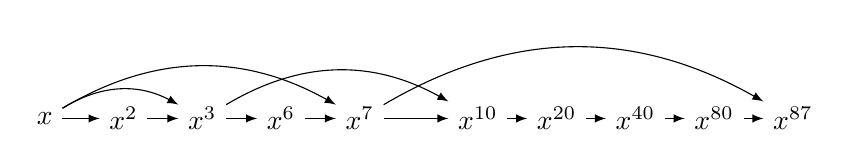
\begin{tikzpicture}
\node (X) at (0,0) {$x$};
\node (X2) at (1,0) {$x^2$};
\node (X3) at (2,0) {$x^3$};
\node (X6) at (3,0) {$x^6$};
\node (X7) at (4,0) {$x^7$};
\node (X10) at (5.5,0) {$x^{10}$};
\node (X20) at (6.5,0) {$x^{20}$};
\node (X40) at (7.5,0) {$x^{40}$};
\node (X80) at (8.5,0) {$x^{80}$};
\node (X87) at (9.5,0) {$x^{87}$};
\draw [->, >=latex](X) -- (X2);
\draw [->, >=latex](X2) -- (X3);
\draw [->, >=latex](X3) -- (X6);
\draw [->, >=latex](X6) -- (X7);
\draw [->, >=latex](X7) -- (X10);
\draw [->, >=latex](X10) -- (X20);
\draw [->, >=latex](X20) -- (X40);
\draw [->, >=latex](X40) -- (X80);
\draw [->, >=latex](X80) -- (X87);
\draw [->, >=latex](X) to [bend left] (X3);
\draw [->, >=latex](X) to [bend left] (X7);
\draw [->, >=latex](X3) to [bend left] (X10);
\draw [->, >=latex](X7) to [bend left] (X87);
\end{tikzpicture}
\end{figure}

\begin{figure}[h]
  \centering
  
  \caption{Graphical representation of $c'_{87}$ (10 multiplications)}
  \label{fig:chain-87-bin}
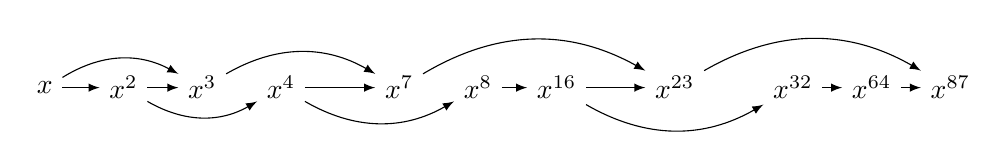
\begin{tikzpicture}
\node (X) at (0,0) {$x$};
\node (X2) at (1,0) {$x^2$};
\node (X3) at (2,0) {$x^3$};
\node (X4) at (3,0) {$x^4$};
\node (X7) at (4.5,0) {$x^7$};
\node (X8) at (5.5,0) {$x^8$};
\node (X16) at (6.5,0) {$x^{16}$};
\node (X23) at (8,0) {$x^{23}$};
\node (X32) at (9.5,0) {$x^{32}$};
\node (X64) at (10.5,0) {$x^{64}$};
\node (X87) at (11.5,0) {$x^{87}$};
\draw [->, >=latex](X) -- (X2);
\draw [->, >=latex](X) to [bend left] (X3);
\draw [->, >=latex](X2) to [bend right] (X4);
\draw [->, >=latex](X2) -- (X3);
\draw [->, >=latex](X4) -- (X7);
\draw [->, >=latex](X3) to [bend left] (X7);
\draw [->, >=latex](X4) to [bend right] (X8);
\draw [->, >=latex](X7) to [bend left] (X23);
\draw [->, >=latex](X8) -- (X16);
\draw [->, >=latex](X16) -- (X23);
\draw [->, >=latex](X16) to [bend right] (X32);
\draw [->, >=latex](X32) -- (X64);
\draw [->, >=latex](X64) -- (X87);
\draw [->, >=latex](X23) to [bend left] (X87);
\end{tikzpicture}
\end{figure}



Let us assume that the efficiency of an exponentiation algorithm is proportional
to the number of multiplications it requires. This assumption looks reasonable 
when the data size is bounded (for instance : machine integers, arithmetic modulo $m$, etc.). 
Let us define the \emph{length} of a chain $c$ as its number $|c|$ of exponents
(without counting the initial $1$). 
This length is the number of multiplications needed for 
computing the $x^i$s by applying the following algorithm:

\begin{quote}
For any item $i$ of $c$ (but the first one), there exists $j$ and $k$ in $c$, where
$i=j+k$, and $x^j$ and $x^k$ are already computed.

Thus, compute $x^i = x^j \times x^k$.
\end{quote}

In our little example, we have 
$|c_{87}| = 9 < 10 = |c'_{87}|$. 
In the rest of this chapter, we will try to focus on the following aspects:
\begin{itemize}
\item Define a representation of addition chains that allows to compute
  efficiently $x^n$ in any monoid, for quite large exponents $n$;
\item Certify that our representation of chains is correct, 
    \emph{i.e.}, determines a computation of $x^n$ for a given $n$;
\item Define and certify functions for automatically  generating 
    correct and shortest as possible chains.
\end{itemize}

In a previous work~\cite{DBLP:journals/ita/BrlekCHM95, DBLP:conf/tapsoft/BrlekCS91,AdditionsContrib},  addition chains were represented so as to allow
efficient computations of powers and certification of a family of
automatic chain generators.
  We present here a new implementation that takes into account some
advances in the way we use \coq{}: generalized rewriting, type classes,
parametricity, etc.


\subsection{A type for addition chains}

Let us recall that we want to represent some algorithms of the form
described in section~\ref{pow-17-let-in}, but avoiding to represent
intermediate results by \textbf{let-in}  constructs.
We describe below the main design choices we made:

\begin{itemize}
\item Continuation Passing Style (CPS) 
\index{coq}{Continuation Passing Style (CPS)} \cite{reynolds93}
is a way to make explicit the 
     control in the evaluation of an expression, in a purely functional way. 
    For every intermediate computation step, the result is sent
    to a \emph{continuation} that executes the further continuations.
   When the continuation is a lambda-abstraction, its bound variable 
   gives a \emph{name} to this result


  
\item Like in Parametric Higher Order Abstract Syntax (PHOAS)~\cite{PHOAS}, \index{coq}{Parametric Higher-Order Abstract Syntax (PHOAS)}
     the local variables associated to intermediate results are
     represented by variables of  type $A$, where $A$ is the underlying type
  of the considered monoid.
\end{itemize}


\subsubsection{Definition}
\label{computation-def}
Let  \texttt{A} be some type;  a \emph{computation} on \texttt{A} is 
\begin{itemize}
\item  either a final step, returning some value of type \texttt{A}
\item or the multiplication of two values of type  \texttt{A}, with a  \emph{continuation}
  that takes as argument the result of this multiplication, then starts a new
  computation.
\end{itemize}
  
  In the following inductive type definition, the intended meaning 
  of the construct (\texttt{Mult $x$ $y$ $k$})  is \emph{``multiply \texttt{x} with
\texttt{y}, then send  the result of this multiplication to 
  the continuation  \texttt{k}''}.



From Module~\href{../theories/html/additions.Addition_Chains.html}{additions.Addition\_Chains}

\inputsnippets{Addition_Chains/computationDef}


\subsubsection{Monadic notation}

\index{additions}{Types!computation}

The following \emph{monadic} 
notation makes terms of type \texttt{computation} look like
expressions of a small programming language dedicated to sequences of multiplications.
Please look at \emph{CPDT}~\cite{chlipalacpdt2011} for more details on monadic notations in \coq.
\label{monadic-mult}

\inputsnippets{Addition_Chains/monadicComputation}

The \texttt{computation} type family is able to express sharing of intermediate computations. For instance, the computation of $2^7$ depicted in Figure~\ref{fig:dag7} is described by  the following term:

\inputsnippets{Addition_Chains/comp128}

\begin{figure}[h]
  \centering
  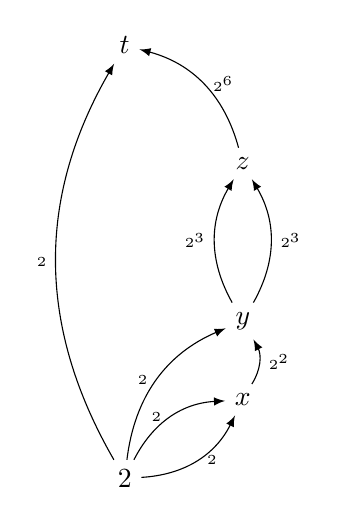
\begin{tikzpicture}
  \node (leaf) at (2,0){\texttt{$2$}};
  \node (x2) at (3.5,1){\texttt{$x$}};
  \node (x3) at (3.5,2){\texttt{$y$}};
 \node (x6) at (3.5,4){\texttt{$z$}};
  \node  (root) at (2,5.5) {\texttt{$t$}};
\draw [->, >=latex, bend left] (leaf) to  node[midway, left] {\tiny{$2$}} 
 (root);
  \draw [->, >=latex,bend left] (leaf) to  node[midway, left] {\tiny{$2$}}  
(x2);
  \draw [->, >=latex,bend right] (leaf) to  node[midway, right] {\tiny{$2$}} 
 (x2);
 \draw [->, >=latex,bend left] (leaf) to  node[midway, left] {\tiny{$2$}} 
 (x3);
\draw [->, >=latex,bend right] (x2) to  node[midway, right] {\tiny{$2^2$}} 
 (x3);
\draw [->, >=latex,bend left] (x3) to  node[midway, left] {\tiny{$2^3$}} 
 (x6);
\draw [->, >=latex,bend right] (x3) to  node[midway, right] {\tiny{$2^3$}} 
 (x6);
\draw [->, >=latex, bend right] (x6) to  node[midway, right] {\tiny{$2^6$}} 
 (root);
  \end{tikzpicture}
  \caption{The dag associated to a computation of $2^7$}
  \label{fig:dag7}
\end{figure}

\subsubsection{Definition}
\label{chain-def}

Thanks to the  \texttt{computation} type family, we can associate a type
to the kind of computation schemes described in Figures~\ref{fig:chain-87-eucl} and ~\ref{fig:chain-87-bin}.

We define 
 \emph{addition chains} (in short  \emph{chains}) as functions that map
 any
 type \texttt{A} and any value \texttt{a} of type \texttt{A}  into a computation 
on \texttt{A}:

\index{additions}{Types!chain@chain (addition chains)}

\inputsnippets{Addition_Chains/chainDef}


Thus, terms of type \texttt{chain} describe polymorphic 
exponentiation algorithms. 


For instance, Fig~\vref{fig:C87} shows a definition of the chain  of Figure~\ref{fig:chain-87-eucl}, for the exponent $87$.
Note that, like in PHOAS, bound variables associated with the 
intermediary results are \coq{} variables of type $A$.
\begin{figure}[h]
  \centering
  \inputsnippets{Addition_Chains/C87}
   \caption{A chain for raising x to its $87$-th power}
  \label{fig:C87}
\end{figure}



The structure of the definition of types \texttt{computation}   and \texttt{chain} suggest that basic definitions over \texttt{chain} will have the following structure:
\begin{itemize}
\item A recursive function on type \texttt{computation $A$} (for a given
    type $A$)
\item A main function on type \texttt{chain} that calls the previous one on 
any \texttt{$A$:Type}.
\end{itemize}

For instance, the following function computes the length of any chain,
\emph{i.e.}, the number of multiplications of the associated computation.
Note that the function \texttt{chain\_length} calls the auxiliary function
\texttt{computation\_length}, with the variable \texttt{A} instantiated to the singleton type  \texttt{unit}. 

Any other type in \coq{} would have fitted our needs, but \texttt{unit} and
its unique inhabitant \texttt{tt} was the simplest  solution.

\label{C87-length}

\inputsnippets{Addition_Chains/chainLength}

\subsection{Chains as a (small) programming language}

The \texttt{chain} type can be considered as a tiny programming language dedicated to compute powers in any \texttt{EMonoid}. Thus, we have to define a semantics for this language. This semantics is defined in two parts:
\begin{itemize}
\item A structurally recursive function,  --- parameterized with an \texttt{EMonoid} \texttt{M} on a given type \texttt{A} ---, that computes the value associated with any computation on \texttt{M}
\item A polymorphic function that takes as arguments  a  chain \texttt{c},
 a type \texttt{A},  an \texttt{EMonoid} on \texttt{A}, and 
   a value \texttt{x:A},
  then executes the computation \texttt{(c A x)}.
\end{itemize}

\inputsnippets{Addition_Chains/chainExecute}




\subsubsection*{Examples:} 
The following interactions show how to apply the chain \texttt{C87} 
for exponentiation within two different monoids:


\inputsnippets{Addition_Chains/C87Apply}

\index{additions}{Projects}
\begin{project}
Study how  to compile efficiently such data structures.

\end{project}

\index{additions}{Projects}
\begin{project}
Define a function which returns the sequence of operations defined by a chain.
For instance, the chain \texttt{C87} of Figure \ref{fig:C87} can be represented as a 
list containing terms of the form \texttt{($i$, Add $j$ $k$)} whenever the associated computation contains the operation $x^i=x^j\times x^k$.

\inputsnippets{Trace_exercise/traceC87}

\textbf{Note} A first solution (in ~\href{../theories/html/additions.Trace_exercise.html}{additions.Trace\_exercise}) consists in the definition of 
a (non-associative) multiplication over a type of trace, and apply the function
\texttt{chain\_execute} as if it were computing a power of \texttt{(1,Init)}.

\end{project}

\subsubsection{Chain correctness and optimality}

A chain is said to be \emph{correct} with respect to a positive
integer \texttt{p} if its execution in any monoid computes $p$-th powers.

\label{chain-correct-def}

\inputsnippets{Addition_Chains/chainCorrect}



\begin{definition}
A chain $c$ is \emph{optimal} for a given exponent $p$ if its length is less 
than or equal to
the length of any chain correct for $p$.  
\end{definition}

\inputsnippets{Addition_Chains/optimalDef}

 \section{Proving a chain's correctness}
\label{chain-correctness-sect}
In this section, we present various ways of proving that a given chain is 
correct w.r.t. a given exponent. First, we just try to apply 
the definition in Section~\vref{chain-correct-def}, but this method is very 
inefficient, even for small exponents. In a second step, we use more sophisticated techniques such as reflection and parametricity. Automatic generation of correct chains will be treated in Sect.~\vref{chain-generation}.

\subsection{Proof by rewriting}
Let us show how to prove  the correctness of some chains, using
the \texttt{EMonoid} laws shown in Sect.~\vref{EMonoid-def}. 

\inputsnippets{Addition_Chains/slowTac}

Unfortunately, this approach is terribly inefficient, even for quite small exponents:

\inputsnippets{Addition_Chains/slowC87Correct}


In addition to this big computation time, this approach 
generates a huge proof term. Just try to execute the command 
``\texttt{Print C87\_ok}'' to get a measure of its size.
In order to understand this poor performance, let us consider an intermediate
subgoal of the previous proof generated after a sequence of unfoldings and simplifications. This goal is presented below.
\begin{figure}[h]
  \centering
\inputsnippets{Addition_Chains/WhySoSlow}  
  \caption{A big goal}
  \label{fig:big-goal}
\end{figure}



This inefficiency certainly comes from the cost of setoid rewriting.
At every application of an \texttt{EMonoid} law, the system must
verify that the context of this rewriting is compatible  with the equivalence
relation associated with the current \texttt{EMonoid}.
The rest of this chapter is devoted to the  presentation of more efficient 
 methods for proving chain correctness.
 

\subsection{Correctness proofs by reflection}
\label{reflection-section}
\index{coq}{Proofs by reflection}
Instead of letting the tactic \texttt{rewrite} look for contexts in which
setoid rewriting is possible, we propose to use (deterministic) computations for
obtaining a ``canonical'' form for terms generated from a variable \texttt{x}
by constructors associated with monoid multiplication and neutral element.

The reader will find general explanations about proofs by reflection in \coq{},
for instance in Chapter 16 of Coq'Art\cite{BC04} and the numerous examples (including the \texttt{ring} tactic) 
in \coq's reference manual.


\subsubsection{How does reflection work}
Let us consider again the subgoal on Fig.~\vref{fig:big-goal}, the conclusion of which has the form \texttt{|$a_1\,==\,a_2$|}, where \texttt{|$a_1$|} and
\texttt{|$a_2$|} are terms of  type \texttt{A}.
Instead of spending space and time in setoid rewritings, we would like to
normalize the terms \texttt{|$a_1$|} and \texttt{|$a_2$|} and verify that 
the associated normal forms are equal.

Defining such a normalization function is possible on an inductive type.
The following type describes expressions composed of monoid operations and inhabitants of a given type $A$.

\pagebreak
\inputsnippets{Addition_Chains/MonoidExp}

Thus, the main steps of a correctness proof of a given chain, \emph{e.g.},
\texttt{C87} will be the following ones:
\begin{enumerate}
\item generate a subgoal as in Fig.~\vref{fig:big-goal},
\item express each term of the equivalence as the image of a term
     of type \texttt{Monoid\_Exp $A$},
\item normalize both terms and verify that their normal forms are equal.
\end{enumerate}

The rest of this section is devoted to the definition of the normalization 
function on \texttt{Monoid\_Exp $A$}, and the proofs of lemmas that
link equivalence on type \texttt{A} and equality of normal forms
of terms of type \texttt{Monoid\_Exp $A$}.


\subsubsection{Linearization function}

The following functions help to transform any term of type
\texttt{Monoid\_Exp $A$} into a flat ``normal form''.

\inputsnippets{Addition_Chains/flattenDef}

\subsubsection{Interpretation function}

The function \texttt{eval} maps any term of type \texttt{Monoid\_Exp $A$}
into a term of type \texttt{$A$}.

\inputsnippets{Addition_Chains/evalDef}


The following two lemmas relate the linearization function \texttt{flatten}
with the interpretation function \texttt{eval}.

\inputsnippets{Addition_Chains/flattenValid}
\inputsnippets{Addition_Chains/flattenValid2}

\subsubsection{Transforming a multiplication into a tree}
Let us now build a tool for building terms of type  (\texttt{Monoid\_Exp $A$}) out
of terms of type \texttt{A} containing multiplications of the form 
\Verb|(_ * _)%M| and the variable \texttt{one}. 
In fact, what we want to  define is an inverse of the function \texttt{flatten}.

Since \texttt{mult\_op} is not a constructor (see Sect.~\ref{op-classes}), 
the transformation of  
a product of type \texttt{A} into a term of type \texttt{Monoid\_Exp A}
is done with the help of a tactic:

\inputsnippets{Addition_Chains/modelTac}

For instance, the term \texttt{(x * x * x * (x * x * x) * x)} is
transformed by \texttt{model} in the following term of type \texttt{Monoid\_Exp $A$}

\begin{Coqsrc}
(eval M
   (Mul_node
     (Mul_node 
        (Mul_node (Mul_node (A_node x) (A_node x)) (A_node x))
        (Mul_node (Mul_node (A_node x) (A_node x)) (A_node x))) 
     (A_node x)))  
\end{Coqsrc}


\subsection{Reflection tactic}
The tactic \texttt{monoid\_eq\_A} converts a goal of the form 
(\texttt{E\_eq $X$ $Y$}), where
\texttt{$X$} and \texttt{$Y$} are terms of type $A$, into
(\texttt{E\_eq (eval M  (model X)) (eval M  (model Y))}). This last goal is intended to be solved thanks 
to the lemma \texttt{flatten\_valid\_2}.

\inputsnippets{Addition_Chains/monoidEqTac}

\subsubsection{Main reflection tactic}

The tactic \texttt{reflection\_correct\_tac} tries to prove a chain's 
correctness by a comparison of two terms of type \texttt{Monoid\_Exp $A$}:
one being obtained from the chain's definition, the other one by expansion
of the naive exponentiation definition.

\inputsnippets{Addition_Chains/reflectionCorrectTac}

\subsubsection{Example}
The following dialogue clearly shows the efficiency gain over naive setoid rewriting.

\inputsnippets{Addition_Chains/reflectionDemo}


This tactic is not adapted to much bigger exponents. In \linebreak
 Module~\href{../theories/html/additions.Euclidean_Chains.html}{Euclidean\_Chains},
 for instance, we tried to apply this tactic for proving the correctness 
of a chain associated with the exponent $45319$. 
 We had to interrupt the prover, which 
was trying to build a linear tree of $2\times  45319 + 1$ nodes!
Indeed, using \texttt{reflection\_correct\_tac} is like doing a 
symbolic evaluation of an inefficient (linear) exponentiation algorithm.

In the next section, we present a solution that avoids doing such a lot of computations.

\subsection{Chain correctness for ---practically --- free!}
\label{correctness-for-free}

% Let us consider again the chain \texttt{C87} of Fig.~\vref{fig:C87}.
% Every bound variable of type \texttt{A} is either the argument \texttt{x}
% or a variable introduced by the abstraction corresponding to the
% continuation argument of constructor \texttt{Mult} (hidden by the monadic notation). Thus, it seems obvious that during the execution of some  computation
% \texttt{C87 A a}, each of this variable will be bound to some power of 
% \texttt{a}. 

% Thus, we would like to prove that  every chain \texttt{c} has this property,
% which would be a great step for proving any chains's correctness.



\subsubsection{About parametricity}
\index{coq}{Parametricity}
Let us now present another tactic for proving chain correctness,
in the tradition of works on \emph{parametricity} and its use for 
proving properties on programs.
Strachey~\cite{Strachey:2000:FCP:609150.609208}
explores the nature of \emph{parametric
polymorphism}: ``\emph{Polymorphic functions behave uniformly for all types}''
then Reynolds~\cite{REYNOLDS83} formalizes this notion through binary relations.
Wadler~\cite{Wadler1989}, then Cohen \emph{et al.}~\cite{Cohen2013}
use this relation for deriving
 theorems about functions that operate on parametric
polymorphic types.

Let us look again at the definitions of type family \texttt{computation}
and the type \texttt{chain}:

\inputsnippets{Addition_Chains/computationDef,
  Addition_Chains/chainDef}

Let $c$ be a closed term of type 
\texttt{chain}; $c$ is  of the form \linebreak
\texttt{fun (A:Type)(a:A) => $t_a$}, where $t_a$ is a term of type
\texttt{@computation A}.
\label{obvious-remark}
Obviously,  in every subterm of {$t_a$} of type \texttt{A}, 
the two first arguments of constructor \texttt{Mult} or the
argument of \texttt{Return} are either \texttt{a} or a variable 
introduced as the formal argument of a continuation \texttt{k}.
In effect, there is no other way to build terms of type \texttt{A} in the considered context.

\index{coq}{Plug-ins!paramcoq}

Marc Lasson's \textbf{paramcoq} plug-in~(available as  \texttt{opam} package 
\texttt{coq-paramcoq}) generates  a family of binary relations definitions
from \texttt{computation}'s definition.

\pagebreak

\inputsnippets{Addition_Chains/paramDemo}



Let $A$ and $B$  be two types, and $R: A \arrow B \arrow \typesort$ 
a relation.
Two computations \texttt{cA: @computation A} and \texttt{cB: @computation B}
are related \emph{w.r.t.} \texttt{computation\_R} if every pair of 
arguments of \texttt{Mult} and \texttt{Return} at the same position 
are related \emph{w.r.t.} \texttt{R}.


\subsubsection{Definition}
A chain $c$ is \emph{parametric} if it has the same behavior for any
pair of types $A$  and $B$, any relation $R$
between  $A$ and $B$ and any $R$-related pair of 
arguments $a$ and $b$:

\inputsnippets{Addition_Chains/parametricDef}

\subsubsection{How to use these definitions?}
Let us use parametricity for proving easily 
a given chain's correctness.
In other words, 
let $c$ be a chain and \texttt{$p$:positive} be a given exponent.
Consider some instance of \texttt{EMonoid} over a type $A$.
We want to prove that the application of the chain $c$ to 
any value $a$ of type $A$ returns the value \texttt{$a^p$}.

We first use \coq's computation facilities for ``guessing'' the exponent associated with any given chain. It suffices to instantiate ``monoid multiplication'' with addition on positive integers.

\inputsnippets{Addition_Chains/theExponent}

We show how to \emph{prove} that  a given  chain $c$,
applied to any $a$, really computes $a^p$, where $p=\textrm{the\_exponent}\;c$.
Parametricity allows us to compare executions on any monoid $M$ 
with executions on \texttt{NatPlus}.
Let us consider the  mathematical relation 
$\{(x,n)\in M\times\mathbb{N}\,|\, 0<n \wedge x=a^n\}$.

\inputsnippets{Addition_Chains/powerR}

First, we prove the following lemma, that relates \texttt{computation\_R}
with the result  of the  executions of the corresponding computations:

\inputsnippets{Addition_Chains/powerRRef}

Thus, if \texttt{$c$:chain} is parametric, this refinement lemma allows us
to prove a correctness result:

\inputsnippets{Addition_Chains/paramCorrectnessNat}

A similar result can be proven with the exponent in \texttt{positive}.
First we instantiate the parameter \texttt{R} of \texttt{computation\_R},
with the relation that links the representations of natural numbers
on respective types \texttt{nat} and \texttt{positive}.
Then we use our lemmas for rewriting under the assumption that the
considered chain is parametric. Please note how our approach is related with
\emph{data refinement} (see also~\cite{Cohen2013}).
The reader may also consult a survey by D. Brown on the most important contributions to 
the notion of parametricity~\cite{DanBrown-survey}.

\inputsnippets{Addition_Chains/exponentPosToNat}
\inputsnippets{Addition_Chains/exponentPosOfNat}
\inputsnippets{Addition_Chains/paramCorrectness}


Lemma \texttt{param\_correctness} suggests us a method for verifying 
that a given chain $c$ is correct \emph{w.r.t.} some positive exponent $p$:

\begin{enumerate}
\item Verify that $c$ is parametric.
\item Verify that $p$ is equal to (\texttt{the\_exponent $c$}).
\end{enumerate}

\subsubsection{How to prove a chain's parametricity}
Despite the apparent complexity of \texttt{computation\_R}'s definition,
it is very simple to prove that a given chain is parametric. The following tactics
proceed as follows:

\begin{enumerate}
\item Given a chain $c$, consider two types \texttt{A} and
\texttt{B}, and any relation \texttt{R:A->B->Prop}, 
\item Push into the context declarations of \texttt{a:A}, \texttt{b:B}
and an hypothesis assuming \texttt{R a b}.
\item Then the tactic crosses in parallel the terms (\texttt{c A a}) and
(\texttt{c B b}) (of the same structure),
\begin{itemize}
\item On a pair of terms of the form 
\texttt{Mult xA yA (fun zA => tA)} and \linebreak \texttt{Mult xB yB (fun zB => tB)}, the tactic checks whether 
   \texttt{R xA xB} and \texttt{R yA yB} are already assumed in the context,
 then  pushes into the context the declaration of \texttt{zA} and \texttt{zB}
and the hypothesis \linebreak \texttt{Hz: R zA zB}, then crosses the terms \texttt{tA} and
 \texttt{tB}
\item On a pair of terms  of the form   (\texttt{Return xA}) and (\texttt{Return xB}),
 the tactic just checks whether (\texttt{R xA xB}) is assumed.
\end{itemize}

\end{enumerate}

The tactic itself is simpler than its explanation. 

\inputsnippets{Addition_Chains/parametricTac}

\subsubsection{Proving a chain's correctness}
\label{C87-param-ok}
Finally, for proving that a given chain $c$ is correct with respect to an exponent $p$, it suffices to check that $c$ is parametric, and
to apply the lemma \texttt{param\_correctness}. 
The reader will note how this computation-less method is much more efficient
than our reflection tactic.

\inputsnippets{Addition_Chains/paramChainCorrect}

\subsubsection{Remark}
For the reasons exposed in Section~\vref{obvious-remark}, 
it seems obvious that any well-written chain is parametric.
Unfortunately, we cannot prove this property  in \coq{},
for instance by induction on \texttt{c}, 
since \texttt{chain} is a product type and not an inductive type.

\inputsnippets{Addition_Chains/VeryBad,Addition_Chains/VeryBad2}

Given this situation, we could  admit (as an axiom) that 
any chain is parametric. Nevertheless, if a chain is under the form of a 
closed term, using \texttt{parametric\_tac} is so efficient than we prefer to 
 avoid
a shameful introduction of an axiom in our development.

\section{Certified chain generators}
\label{chain-generation}

In this section, we are interested in the \emph{correct by construction} paradigm.
We just want to give a positive exponent to \coq{} and get a (hopefully)  correct and  efficient chain for this exponent.

We first define the notion of \emph{chain generator}, then present a certified generator that simulates the binary exponentiation algorithm. Last, we present a better chain generator based on integer division.


\subsection{Definitions}

We call \emph{chain generator} any function that takes as argument 
any positive integer and returns a chain.
A generator $g$  is \emph{correct} it it returns a correct chain
for any exponent.

\inputsnippets{Addition_Chains/generatorDef}

Correct generators can be used for computing powers 
on the fly, thanks to the following functions:

\inputsnippets{Addition_Chains/cpowerDef}


Note also that the use of chain generators is independent from  the techniques presented in Sect.~\ref{chain-correctness-sect}:
Designing an efficient and correct chain generator may be a long and hard task.
On the other hand, once a generator is certified, we are assured of the correctness of  
all its outputs.
Finally, we say that a generator $g$ is \emph{optimal} if it returns chains whose length are less than or
equal to any chain returned by any correct generator:

\inputsnippets{Addition_Chains/optimalGenerator}

\subsection{The binary chain generator}

Let us reinterpret the  binary exponentiation algorithms in the framework 
of addition chains.
Instead of directly computing $x^n$ for some base $x$ and exponent $n$,
we build chains that describe the computations associated with the binary exponentiation method.
Not surprisingly, this chain generation will be described in terms of recursive
functions, once the underlying monoid is fixed.

As for the ``classical'' binary exponentiation algorithm,
we define an auxiliary computation generator for  the
product of an accumulator $a$ with an arbitrary power of some value $x$.

\inputsnippets{Addition_Chains/binaryChain}




\subsubsection{Proof of \texttt{binary\_chain}'s correctness}

Let us now prove that \texttt{binary\_chain} always returns correct chains.
First, due to the structure of this generator's definition, we study the
properties of the auxiliary functions that operate \emph{on a given monoid $M$}.

\inputsnippets{Addition_Chains/binaryPowerProofa}
\inputsnippets{Addition_Chains/binaryPowerProofb}
\inputsnippets{Addition_Chains/binaryPowerProofc}
\inputsnippets{Addition_Chains/binaryPowerProofd}
\inputsnippets{Addition_Chains/binaryGeneratorOk}

\subsubsection{The binary method is not optimal}

It is easy to prove by contradiction  that the binary method is not the most efficient 
for computing powers. 

\inputsnippets{Addition_Chains/nonOpt}

\index{additions}{Exercises}
\begin{exercise}
Prove that for any positive integer $p$,  the length of any optimal chain 
for $p$ is less  than twice the number of digits of the binary representation of $p$.
\end{exercise}


\section{Euclidean Chains}
\label{euclide-sect}
\index{maths}{Euclidean addition chains}
In this section, we present an efficient chain generator. The chains built by this generator
are never longer than the chains built by the binary generator. Moreover, for an 
infinite number of exponents, the chains it builds are strictly shorter than the chain
returned by \texttt{binary\_chain}. 
Euclidean chains are based on the following idea: 
\begin{quote}
For generating a chain that computes $x^n$, one may choose some natural number
$0<p<n$, and build a chain that computes first $x^p$ \textbf{then} uses this value
for computing $x^n$. 
\end{quote}

For instance, a  computation of $x^{42}$ can be decomposed into a computation 
of $y=x^3$, then a computation of $y^{14}$. The efficiency of the chain built with this
methods depends heavily on the choice of $p$. See~\cite{DBLP:journals/ita/BrlekCHM95} for details.

Considering chain generators and their correctness, we may consider the dual of 
decomposition of exponents: we would like to write \emph{composable} correct 
chain generators. For instance, we want to build some object that, ``composed''  
with any correct chain for $n$, returns a correct chain for $3n$.

\paragraph{Note:}
All the \coq{} material described in this section is available on 
 Module~\href{../theories/html/additions.Euclidean_Chains.html}{additions/Euclidean\_Chains.v}

\subsection{Chains and continuations : f-chains}


Please consider the following small example:

\inputsnippets{Addition_Chains/C3Example}


The execution of this chain on  some value $x:A$ stops after 
computing \texttt{$x^3$}, because of the \texttt{Return} ``statement''.
However, we would like to compose the instructions of \texttt{C3} 
with a chain for another exponent $n$, in order to generate a chain for 
the exponent $3\times n$.

  The solution we present is based on functional programming and the concept of continuation.



\subsubsection{Type definition of  f-chains}

Let us   consider \emph{incomplete} or \emph{open} chains.
Such an object waits for another chain to resume  a computation.

Figure~\ref{fig:F3-as-dag} represents an  f-chain associated with the exponent $3$, as a dag with an input and one output the edges of which are depicted as thick arrows.

\begin{figure}[h]
  \centering
  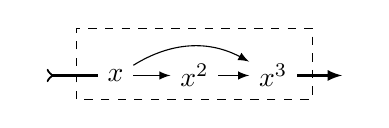
\begin{tikzpicture}
  \node (entree) at (0,0) {};
  \node (X) at (1,0) {$x$};
\node (X2) at (2,0) {$x^2$};
  \node (X3) at (3,0) {$x^3$};
\node (sortie) at (4,0) {};
\draw [>-,   thick](entree) -- (X);
\draw [->, >=latex, ](X) -- (X2);
\draw [->, >=latex, ](X2) -- (X3);
\draw [->, >=latex,  thick](X3) -- (sortie);
\draw [->, >=latex](X) to [bend left] (X3);
\draw[dashed] (0.5,-0.3) rectangle (3.5,0.6);
  \end{tikzpicture}
  \caption{Graphical representation of \texttt{F3}}
  \label{fig:F3-as-dag}
\end{figure}

In other words, this kind of objects can be considered as \emph{functions}
from chains to chains. So, we called their type \texttt{Fchain}.



First, we define a type of \emph{continuations},
\emph{i.e.},  functions  that wait for some value $x$, then 
build  a computation for raising {$x$} to some  given exponent.
An \texttt{f-chain} is just a polymorphic function that combines  a 
continuation and an element into a computation.

\inputsnippets{Euclidean_Chains/FchainDef}

\subsubsection{Examples}

Let us define a chain for computing the cube of some $x$, then sending 
the result to a continuation $k$.

\inputsnippets{Euclidean_Chains/F3Def}

Any f-chain can be converted into a chain by the help of the following function:

\inputsnippets{Euclidean_Chains/F2C}


In the rest of this chapter, we will use two other f-chains, respectively associated with the exponents $1$ and $2$. Chains \texttt{F1}, \texttt{F2} and
\texttt{F3} will form a basis to generate  chains for many exponents
by \emph{composition of correct functions}.

\inputsnippets{Euclidean_Chains/F1F2}


\subsubsection{F-chain application and composition}

The following definition allows us to consider any value {$f$} 
of type 
\texttt{Fchain} as a function of type \texttt{chain $\arrow$ chain}.

\inputsnippets{Euclidean_Chains/Fapply}


In a similar way, \emph{composition} of \texttt{f-chain}s is easily defined
(see Figure~\vref{fig:Fcompose}).

\inputsnippets{Euclidean_Chains/Fcompose}

\inputsnippets{Euclidean_Chains/F1Neutral}



\begin{figure}[h]
  \centering
  \begin{tikzpicture}
 \node (input1)  at (0,0) {};  
 \node [draw] (F1)  at (1,0) {$f_1$};  
 \node (output1)  at (2.0,0) {};  
 \node (input2)  at (2.6,0) {};  
 \node [draw] (F2)  at (3.5,0) {$f_2$};  
 \node (output2)  at (4.5,0) {};  
 \draw [>-,   thick](input1) -- (F1);
 \draw [->, >=latex, thick](F1) -- (output1);
\draw [dotted, ](output1) -- (input2);
\draw [>-,   thick](input2) -- (F2);
\draw [->, >=latex, thick](F2) -- (output2);
\draw[dashed] (0.4,-1) rectangle (4,1);
  \end{tikzpicture}
  \caption{Composition  of f-chains $f_1$ and $f_2$ (\texttt{Fcompose})}
  \label{fig:Fcompose}
\end{figure}
\subsubsection{Examples}

The following examples show that the apparent complexity of the previous 
definition is counterbalanced with the simplicity of using \texttt{Fapply}
and \texttt{Fcompose}.

\inputsnippets{Euclidean_Chains/F9Def}
\inputsnippets{Euclidean_Chains/F9Ok}


\begin{figure}[h]
  \centering
  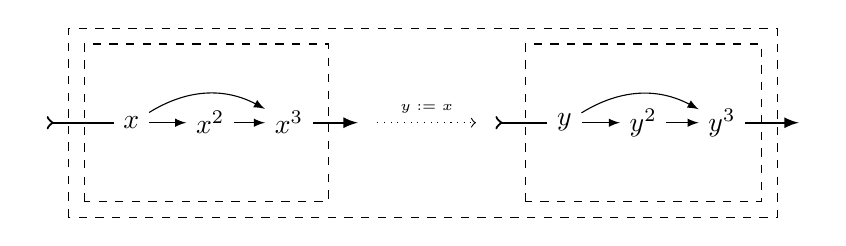
\begin{tikzpicture}

 \node (inputx)  at (-0.2,0) {};  
\node (x)  at (1,0) {$x$};  
 \node (x2)  at (2,0) {$x^2$};  
 \node (x3)  at (3,0) {$x^3$};
 \node (output1)  at (4,0) {};  
 \node (inputy)  at (5.5,0) {};  
\node (y)  at (6.5,0) {$y$};  
 \node (y2)  at (7.5,0) {$y^2$};  
 \node (y3)  at (8.5,0) {$y^3$};
 \node (output2)  at (9.6,0) {};  
 \draw [>-,   thick](inputx) -- (x);
 \draw [->,   >=latex](x) -- (x2);
\draw [->,   >=latex](x2) -- (x3);
\draw [->, >=latex](x) to [bend left] (x3);
\draw [->, >=latex, thick](x3) -- (output1);
\draw [->, dotted ](output1) -- (inputy) node [midway, above] {\tiny{$y:=x$}};
\draw [>-,   thick](inputy) -- (y);
 \draw [->,   >=latex](y) -- (y2);
\draw [->,   >=latex](y2) -- (y3);
\draw [->, >=latex](y) to [bend left] (y3);
\draw [->, >=latex, thick](y3) -- (output2);
\draw[dashed] (0.4,-1) rectangle (3.5,1);
\draw[dashed] (6,-1) rectangle (9,1);
\draw[dashed] (0.2,-1.2) rectangle (9.2,1.2);
  \end{tikzpicture}
  \caption{Composition  of F-chains: F9}
  \label{fig:F9}
\end{figure}

Using structural recursion and the operator \texttt{FCompose},
we build a chain for any exponent of the form $2^n$:

\inputsnippets{Euclidean_Chains/Fexp2}


\subsection{F-chain correctness}
Let \texttt{f} be some term of type \texttt{Fchain}, and \texttt{n:nat}.
We would like to say that \texttt{f} is correct \emph{w.r.t.} \texttt{n:nat}
if for any continuation \texttt{k} and \texttt{a}, the application of 
\texttt{f} to \texttt{k} and \texttt{a} computes \texttt{$k(a^n)$}.

\begin{Coqbad}
Module Bad.

Definition Fchain_correct  (n:nat) (f : Fchain) :=
  forall A `(M : @EMonoid A op E_one E_equiv) k (a:A),
    computation_execute op (f A k  a)==
    computation_execute op (k  (a ^ n)).
\end{Coqbad}

Let us now try to prove that \texttt{F3} is correct \emph{w.r.t.} $3$.

\inputsnippets{Euclidean_Chains/BadDefa}
\inputsnippets{Euclidean_Chains/BadDefb}

This failure is due to a lack of an assumption that the continuation
\texttt{k} is \emph{proper} with respect to the equivalence \texttt{equiv}.
Thus, \coq{} is unable to infer from the equivalence 
\texttt{(a * a * a) == (a * (a * (a * E\_one)))} \linebreak that 
(\texttt{k (a * a * a)}) and (\texttt{k (a * (a * (a * E\_one)))}) are 
equivalent computations.



\subsubsection{Definition:} 
\index{coq}{Type classes}
\index{coq}{Type classes!Proper class}
A continuation \texttt{k:Fkont A} is \emph{proper}
if, whenever \linebreak[3] \texttt{x == y} holds, the computations (\texttt{k x}) and 
(\texttt{k y}) are equivalent.

\inputsnippets{Euclidean_Chains/FkontProper}


We are now able to improve our definition of correctness, taking only
proper continuations into account.

\inputsnippets{Euclidean_Chains/GoodFchainCorrect}

\subsubsection{Examples}

Let us show manual correctness proofs of some small f-chains:

\inputsnippets{Euclidean_Chains/F1Ok}

 While proving \texttt{F3}'s correctness, we will have to apply
 the properness hypothesis on \texttt{k}:

\inputsnippets{Euclidean_Chains/F3Ok}

Correctness of \texttt{F2} is proved the same way:

\inputsnippets{Euclidean_Chains/F2Ok}

\subsubsection{Composition of correct f-chains: a first attempt}

We are now looking for a way to generate correct chains for any positive 
number. It seems obvious that we could use \texttt{Fcompose} for building 
a correct f-chain for $n\times p$ by composition of a correct f-chain for 
$n$ and a correct f-chain for $p$.
Let us try to certify this construction:

\inputsnippets{Euclidean_Chains/Bad2a, Euclidean_Chains/Bad2b}


No hypothesis guarantees us that the execution of \texttt{f2} respects the equivalence
\texttt{x == y}.

\inputsnippets{Euclidean_Chains/Bad2c}

 Thus, we need to define also a  notion of properness for f-chains. 
A first attempt would be :

\inputsnippets{Euclidean_Chains/Bad3}



This definition is powerful enough for proving that properness is 
preserved by composition:

\inputsnippets{Euclidean_Chains/Bad3b}

Nevertheless, we had to throw away  this definition of properness:
In further 
developments (Sect.~\vref{Kkonts-section})  we shall  have to compare
executions of the form \texttt{fc A $k_x$ x} and \texttt{fc A $k_y$ y}
where \texttt{x == y} and {$k_x$} and {$k_y$} are 
``equivalent''
but not \emph{convertible} continuations.

\inputsnippets{Euclidean_Chains/Bad3c}

\subsubsection{A better definition of properness}

 The following  generalization will allow us to consider continuations that are
different (according to Leibniz equality) but lead to equivalent
computations and results.

\inputsnippets{Euclidean_Chains/correctProper}

\subsubsection{Examples}
The definition above allows us  to build simply several instances of the class \linebreak
\texttt{Fchain\_proper}:

\inputsnippets{Euclidean_Chains/F1proper}
\inputsnippets{Euclidean_Chains/F2proper}
\inputsnippets{Euclidean_Chains/F3proper}

\subsection{Correctness of chain composition}

The \texttt{Fcompose} operator respects chain correctness and properness.

\inputsnippets{Euclidean_Chains/FcomposeCorrect}
\inputsnippets{Euclidean_Chains/FcomposeProper}

Using chain composition, we get a correct and proper chain for any exponent of the form $2^n$.

\inputsnippets{Euclidean_Chains/Fexp2Correct}
\inputsnippets{Euclidean_Chains/Fexp2Proper}

We are now  able to build chains for any exponent of the form 
$2^k\times 3^p$, using \texttt{Fcompose}. Les us look at a simple example:

\inputsnippets{Euclidean_Chains/F144}


\subsection{Building chains for two distinct exponents : k-chains  \label{Kkonts-section}}

\subsubsection{Introduction}
Not every chain can be built efficiently  with \texttt{Fcompose}.
 For instance, consider the exponent $n= 23 = 3 + 2^4 + 2^2$. 

One may attempt to define a new operator  for combining f-chains for 
$n$ and $p$ into an f-chain for $n+p$.

\pagebreak
\inputsnippets{Euclidean_Chains/Fplus}

Unfortunately, our construct is still very inefficient, since it results in 
duplication of computations, as shown by the normal form of \texttt{F23}.


\inputsnippets{Euclidean_Chains/Fplusb}

We observe that the variables \texttt{x3} and \texttt{x7} are 
useless, since
they will have the same value as \texttt{x1}. Likewise, computing
\texttt{x8} (same value as \texttt{x4}) is a waste of time.

 A better scheme for computing $x^{23}$ would be the following one:

 \begin{enumerate}
 \item Compute $x$, $x^2$, $x^3$, \textbf{and} $x^6 = {(x^3)}^2$, then  $x^7$,
 \item Compute $x^{10} = x^7 \times x^3$, then $x^{20}$
 \item Finally, return  $x^{23} = x^{20} \times x^3$
 \end{enumerate}

In fact, the first step of this sequence  computes \emph{two}
values: $x^7$ and $x^3$, that are re-used by the rest of the computation.

  Like in some programming languages
 that allow  ``multiple values'', like \texttt{Scheme} and \texttt{Common Lisp}, we can  express this feature 
 in terms of continuations that accept two arguments.
Thus, we extend our previous definitions to chains that return two 
different powers of their argument\footnote{The name \texttt{Kchain} comes from previous versions of this development. It may be changed later.}.


\index{coq}{Continuation Passing Style (CPS)}

\inputsnippets{Euclidean_Chains/KchainDef}

\subsubsection{Examples}

The chain \texttt{k3\_1} sends both values $x$ and $x^3$ to its continuation.
Likewise, \texttt{k7\_3} ``returns''  $x^7$ and $x^3$. 

\inputsnippets{Euclidean_Chains/K31}
\inputsnippets{Euclidean_Chains/K73}



\begin{figure}[h]
  \centering
  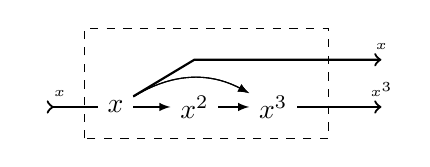
\begin{tikzpicture}
  \node (entree) at (0,0) {};
  \node (X) at (1,0) {$x$};
\node (X2) at (2,0) {$x^2$};
  \node (X3) at (3,0) {$x^3$};
\node (sortieX) at (4.5,0.6) {};
\node(beforeSortieX) at (2,0.6){};
\node (sortieX3) at (4.5,0) {};
\draw [>-,   thick](entree) -- (X) node [near start, above] {\tiny{$x$}};
\draw [->, >=latex, ](X) -- (X2);
\draw [->, >=latex, ](X2) -- (X3);
\draw [->,  thick](X3) -- (sortieX3) node [at end, above] {\tiny{$x^3$}};
\draw [->, >=latex](X) to [bend left] (X3);
\draw [->, >=latex](X) to [bend left] (X3);
%\draw [thick](X) to [bend left] (beforeSortieX)
\draw [->, thick](X) -- (2,0.6) --  (sortieX) node [at end, above] {\tiny{$x$}};
\draw[dashed] (0.6,-0.4) rectangle (3.7,1);
  \end{tikzpicture}
  \caption{Graphical representation of \texttt{K3\_1}}
  \label{fig:K3-1-as-dag}
\end{figure}



\begin{figure}[h]
  \centering
  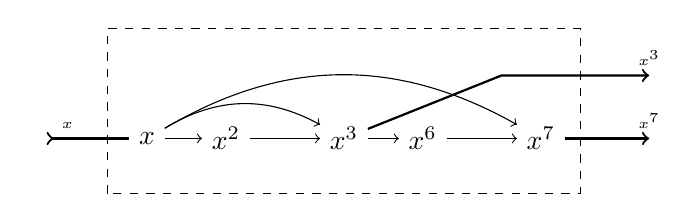
\begin{tikzpicture}
  \node (entree) at (-0.4,0) {};
  \node (X) at (1,0) {$x$};
  \node (X2) at (2,0) {$x^2$};
\node (X3) at (3.5,0) {$x^3$};
  \node (X6) at (4.5,0) {$x^6$};
\node (X7) at (6,0) {$x^7$};
  \draw [>-,   thick](entree) -- (X) node [near start, above] {\tiny{$x$}};
 \draw [->](X) -- (X2);
\draw [->](X2) -- (X3);
\draw [->, bend left](X) to (X3) ;
\draw [->, bend left](X) to (X7) ;
\draw [->](X3) -- (X6) ;
\draw [->](X6) -- (X7) ;
  \node (sortieX7) at (7.5,0) {};
  \node (sortieX3) at (7.5,0.8) {};
 \draw [->,   thick](X7) -- (sortieX7) node [at end, above] {\tiny{$x^7$}};
 \draw [->,   thick](X3) -- (5.5,0.8) -- (sortieX3)  node [at end, above] {\tiny{$x^3$}};
\draw  [dashed] (0.5,-0.7) rectangle (6.5,1.4);
  \end{tikzpicture}
  \caption{Graphical representation of \texttt{K7\_3}}
  \label{fig:K7-3-as-dag}
\end{figure}


\subsubsection{Definitions}

First, we have to adapt to k-chains our definitions of correctness and properness.

\inputsnippets{Euclidean_Chains/KkontDefs}



A k-chain is correct with respect to two exponents $n$ and $p$ 
  if it computes $x ^ n$ and $x ^ p$ for any $x$ in any monoid $M$.

\inputsnippets{Euclidean_Chains/KchainCorrectDef}
  
\subsubsection{Example}
For instance, let us prove that \texttt{k7\_3} is proper and correct for the exponents  $7$ and $3$.

\inputsnippets{Euclidean_Chains/K73Ok}

\subsection{Systematic construction of  correct f-chains and k-chains}

We are now ready to define various operators on f- and k-chains, and prove these
operators preserve correctness and properness. We will also show that
these operators allow to generate easily correct chains for any positive 
exponent. They will be used to generate chains for
numbers of the form $n=bq+r$ where $0\leq r < b$, assuming the previous
construction of correct chains for $r$, $b$ and $q$.
For instance, Figure~\ref{fig:K7-3-decomposition} shows how \texttt{K7\_3} is built
as a composition of \texttt{K3\_1} and \texttt{F2}.



\begin{figure}[h]
  \centering
  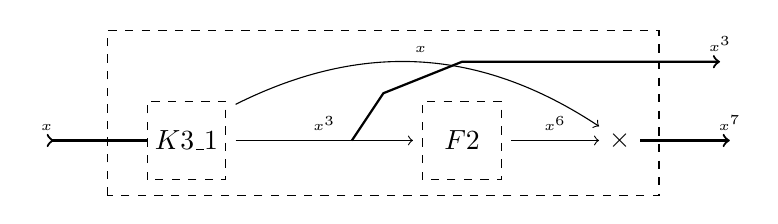
\begin{tikzpicture}
  \node (entree) at (-0.4,0) {};
  \draw [dashed] (1,-0.5) rectangle (2,0.5);
  \node at (1.5,0){$K3\_1$};
  \draw [>-,   thick](entree) -- (1,0) node [at start, above] {\tiny{$x$}};
  \node (sortiex3) at (2,0) {};
  \node (sortiex) at (2,0.4) {};
  \draw [dashed] (4.5,-0.5) rectangle (5.5,0.5);

  \node at (5,0){$F2$};
  \node (entreeF2) at (4.5,0) {};
\node (sortieF2) at (5.5,0) {};
  \draw[->, ] (sortiex3) -- (entreeF2) 
       node [midway, above] {\tiny{$x^3$}};
  \node (sortiex3global) at (7,1) {};
  \node (sortiex3global) at (8.4,1)  {};
  \draw [->, thick, bend left] (3.6,0) -- (4,0.6) -- (5,1) --  node [at end, above]
 {\tiny{$x^3$}} (sortiex3global) ;
  \node (join) at (7,0) {$\times$};
  \draw [->, ] (sortieF2) -- (join)
    node [midway, above] {\tiny{$x^6$}};
\draw [->, bend left] (sortiex) to node [midway, above] {\tiny{$x$}} (join);
    
 \draw [->,   thick](join) -- (8.4,0) node [at end, above] {\tiny{$x^7$}};
% \draw [->,   thick](sortiex3global) --  (8.4,1);
\draw  [dashed] (0.5,-0.7) rectangle (7.5,1.4);
  \end{tikzpicture}
  \caption{Decomposition of  \texttt{K7\_3}}
  \label{fig:K7-3-decomposition}
\end{figure}

\subsubsection{Conversion from k-chains into f-chains}

Any k-chain for $n$ and $p$ can be converted into an f-chain, just by applying it to a continuation that 
ignores its second argument.

\begin{figure}[h]
  \centering
  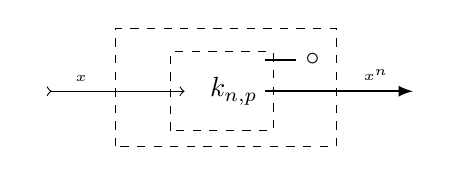
\begin{tikzpicture}
\node (input) at (-0.5,0){};
\node(inputkc) at (1.5,0){};
\node(outputkc1) at (2.5,0){};
\node(outputkc2) at (2.5,0.4){};
\node (ignore) at (3,0.4){{$\circ$}};
\node (output) at (4.4,0){};
\draw [dashed] (1.2,-0.5) rectangle (2.5,0.5) ;
\draw [dashed] (0.5,-0.7) rectangle (3.3,0.8) ;
\node (knp) at (2,0) {$k_{n,p}$};
\draw[>->] (input) -- node [near start, above] {\tiny{$x$}} (inputkc);
\draw[thick, ->,>=latex] (outputkc1) +(-0.1,0) -- (output) node [near end,above] {\tiny{$x^n$}};
\draw[thick] (outputkc2) +(-0.1,0)  -- (ignore);
\end{tikzpicture}
  \caption{The \texttt{K2F (knp)} construction}
  \label{fig:K2F}
\end{figure}

\inputsnippets{Euclidean_Chains/K2FDef}
\inputsnippets{Euclidean_Chains/K2FCorrect}
\inputsnippets{Euclidean_Chains/K2FProper}

\subsubsection{Construction associated with Euclidean division with a positive rest}

Let $n=bq+r$, with $0<r<b$. Then, for any $x$,  $x^n= (x^{b})^q \times x^r$. Thus, we can 
compose an chain that computes $x^b$ and $x^r$ with a chain that raises
any $y$ to its $q$-th power for obtaining a chain that computes $x^n$.


\begin{figure}[h]
  \centering
  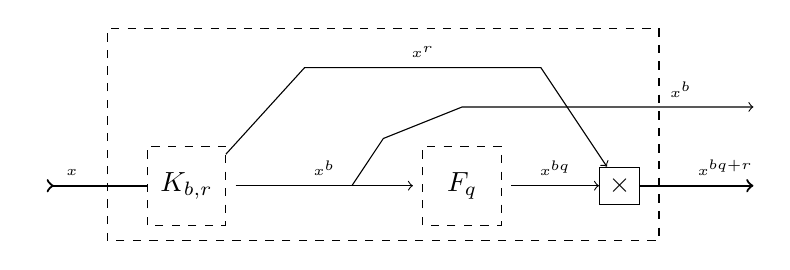
\begin{tikzpicture}
  \node (entree) at (-0.4,0) {};
  \draw [dashed] (1,-0.5) rectangle (2,0.5);
  \node at (1.5,0){$K_{b,r}$};
  \draw [>-,   thick](entree) -- (1,0) node [above, near start] {\tiny{$x$}};
  \node (sortiex3) at (2,0) {};
  \node (sortiex) at (2,0.4) {};
  \draw [dashed] (4.5,-0.5) rectangle (5.5,0.5);
  \node at (5,0){$F_q$};
  \node (entreeF2) at (4.5,0) {};
\node (sortieF2) at (5.5,0) {};
  \draw[->, ] (sortiex3) -- (entreeF2) 
       node [midway, above] {\tiny{$x^b$}};
  %\node (sortiex3global) at (7,1) {};
  \node (sortiex3global) at (7,1)  {};
  \draw [->, , bend left] (3.6,0) -- (4,0.6) -- (5,1) -- node [near end, above] {\tiny{$x^b$}} (8.7,1)  ;
  \node [draw] (multipl) at (7,0) {$\times$};
\draw [->] (2,0.4) to (3,1.5) -- node [midway,above] {\tiny{$x^r$}} (6,1.5) to (multipl);
  \draw [->, ] (sortieF2)  -- (multipl)   node [midway, above] {\tiny{$x^{bq}$}};
 \draw [->,   thick](multipl) -- (8.7,0) node [above, near end] {\tiny{$x^{bq+r}$}};
\draw  [dashed] (0.5,-0.7) rectangle (7.5,2);
  \end{tikzpicture}
  \caption{The KFK combinator}
  \label{fig:KFK}
\end{figure}

\inputsnippets{Euclidean_Chains/KFKDef}
\inputsnippets{Euclidean_Chains/KFKCorrect}
\inputsnippets{Euclidean_Chains/KFKProper}

%\subsection{More certified operators on chains}

\subsubsection{Ignoring the remainder}

Let $n=bq+r$, with $0<r<b$. The following construction computes
$x^r$ and $x^b$, then $x^{bq}$, and finally sends $x^{bq+r}$ to the continuation,
throwing away $x^b$.


\begin{figure}[h]
  \centering
  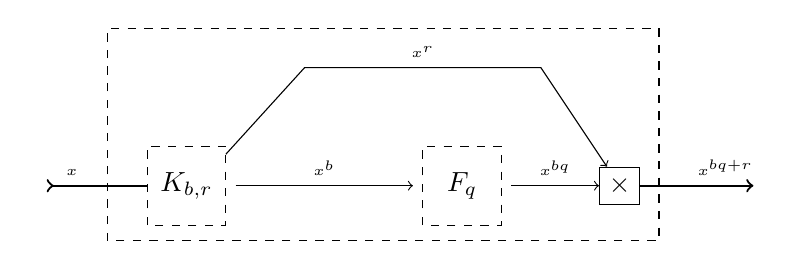
\begin{tikzpicture}
  \node (entree) at (-0.4,0) {};
  \draw [dashed] (1,-0.5) rectangle (2,0.5);
  \node at (1.5,0){$K_{b,r}$};
  \draw [>-,   thick](entree) -- (1,0) node [above, near start] {\tiny{$x$}};
  \node (sortiex3) at (2,0) {};
  \node (sortiex) at (2,0.4) {};
  \draw [dashed] (4.5,-0.5) rectangle (5.5,0.5);
  \node at (5,0){$F_q$};
  \node (entreeF2) at (4.5,0) {};
\node (sortieF2) at (5.5,0) {};
  \draw[->, ] (sortiex3) -- (entreeF2) 
       node [midway, above] {\tiny{$x^b$}};
  %\node (sortiex3global) at (7,1) {};
  %\node (sortiex3global) at (7,1)  {};
  % \draw [->, , bend left] (3.6,0) -- (4,0.6) -- (5,1) -- node [near end, above] {\tiny{$x^b$}} (8.7,1)  ;
  \node [draw] (multipl) at (7,0) {$\times$};
\draw [->] (2,0.4) to (3,1.5) -- node [midway,above] {\tiny{$x^r$}} (6,1.5) to (multipl);
  \draw [->, ] (sortieF2)  -- (multipl)   node [midway, above] {\tiny{$x^{bq}$}};
 \draw [->,   thick](multipl) -- (8.7,0) node [above, near end] {\tiny{$x^{bq+r}$}};
\draw  [dashed] (0.5,-0.7) rectangle (7.5,2);
  \end{tikzpicture}
  \caption{The KFF combinator}
  \label{fig:KFF}
\end{figure}


\inputsnippets{Euclidean_Chains/KFFDef}
\inputsnippets{Euclidean_Chains/KFFCorrect}
\inputsnippets{Euclidean_Chains/KFFProper}

\subsubsection{Conversion of an f-chain into a k-chain}
The following conversion is useful when a chain generation algorithm
needs to build a k-chain for exponents $p$ and $1$:

\inputsnippets{Euclidean_Chains/FKDef}

Like our other combinators, \texttt{FK} respects chain correctness and properness.


\subsubsection{Computing $x^p$ \emph{and} $x^{pq}$}


\begin{figure}[h]
  \centering
  \begin{tikzpicture}
  \node (entree) at (-0.4,0) {};
  \draw [dashed] (1,-0.5) rectangle (2,0.5);
  \node at (1.5,0){$F_p$};
  \draw [>-,   thick](entree) -- (1,0) node [above, near start] {\tiny{$x$}};
  \node (sortiexp) at (2,0) {};
  \draw [dashed] (4.5,-0.5) rectangle (5.5,0.5);
  \node at (5,0){$F_q$};
  \node (entreeF2) at (4.5,0) {};
\node (sortieF2) at (5.5,0) {};
  \draw[->, ] (sortiex3) -- (entreeF2) 
       node [midway, above] {\tiny{$x^p$}};
  \draw [->, , bend left] (3.6,0) -- (4,0.6) -- (5,1) -- node [near end, above] {\tiny{$x^p$}} (7.7,1)  ;
 \draw [->,   thick](sortieF2) -- (7.7,0) node [above, near end] {\tiny{$x^{pq}$}};
\draw  [dashed] (0.5,-0.7) rectangle (6.5,2);
  \end{tikzpicture}
  \caption{The FFK combinator}
  \label{fig:FFK}
\end{figure}

Our last combinator composes a chain for computing $x^p$ with a chain for computing $x^q$ to build a chain for
computing $x^p$ and $x^{pq}$.

\inputsnippets{Euclidean_Chains/FFKDef}
\inputsnippets{Euclidean_Chains/FFKCorrect}
\inputsnippets{Euclidean_Chains/FFKProper}

\subsubsection{A correct-by-construction chain}

A simple example will show us how to build correct chains 
for any positive exponent, using the operators above.

\inputsnippets{Euclidean_Chains/HintKchains}
\inputsnippets{Euclidean_Chains/F87}
\inputsnippets{Euclidean_Chains/F87Correct}

Note that this method of construction still requires some  
interaction from the user. 
In the next section, we build a \emph{function} that maps any 
positive number $n$ into a correct and proper chain for $n$.
Thus correct chain generation will be fully automated.

\subsection{Automatic chain generation by Euclidean division}

The goal of this section is to write a function 
\texttt{make\_chain (p:positive): chain} that builds a correct chain for $p$, using
the Euclidean method above. In other words, we want to get correct chains
by computation. The correctness of the result of this computation should be
asserted by a  theorem:

\begin{Coqsrc}
Theorem make_chain_correct : 
   forall p, chain_correct p (make_chain p).  
\end{Coqsrc}


In the previous section, we  considered two different kinds of objects:
f-chains, associated with a single exponent, and k-chains, associated with two exponents. We would expect that the function \texttt{make\_chain} we want to define and certify is structured as a pair of mutually recursive functions.
 In \coq{} , various ways of building such functions are available:
 \begin{itemize}
 \item Structural [mutual] recursion with \texttt{Fixpoint}
 \item  Using \texttt{Program Fixpoint}
 \item Using   \texttt{Function}.
 \end{itemize}

Since our construction is based on Euclidean division, we could not
define our chain generator by structural recursion. 
For simplicity's sake, we chose to avoid dependent elimination
 and used \texttt{Function}  with a decreasing measure.

 For this purpose, we define a single data-type for associated with
 the generation of F- and K-chains.


We had two slight technical problems to consider:
\begin{itemize}
\item The generation of a k-chain for $n$ and $p$ is meaningful only if $p < n$. Thus, in order to avoid a clumsy  dependent pattern-matching, we chose to represent
     a pair $(n,p)$ where $0<p<n$ by a pair of positive numbers $(p,d)$ where 
     $d=n-p$
\item In order to avoid to deal explicitly with mutual recursion, we
     defined a type called \texttt{signature} for representing both
     forms of function calls.
     Thus, it is easy to define a decreasing measure on type 
     \texttt{signature} for proving termination. 
    Likewise, correctness and properness statements are also indexed by 
    this type.

\end{itemize}

\inputsnippets{Euclidean_Chains/signature}

The following dependently-typed functions will help us to specify  formally
any correct chain generator.
\index{coq}{Dependently typed functions}

\inputsnippets{Euclidean_Chains/dependentlyTypedFuns}

\subsection{Generation of chains using Euclidean Division}

Assume we want to build automatically a correct  f-chain for some 
positive integer $n$.
If $n$ equals to $1$, $3$, or $2^p$ for some positive integer  $p$,
this task is immediate, thanks to the constants \texttt{F1}, 
\texttt{F3} and \texttt{Fexp2}.
Otherwise, like in \cite{DBLP:journals/ita/BrlekCHM95}, we decompose 
$n$ into $bq+r$, where $1<b<n$, and compose the recursively built
chains for $q$ and $r$ on one side, and $q$ on the other side.

The efficiency of this method depends on the choice of $b$.
In \cite{DBLP:journals/ita/BrlekCHM95}, the function that maps $n$ into $b$
is called a \emph{strategy}. 

\vspace{4pt}
\noindent
From ~\href{../theories/html/additions.Strategies.html}{additions.Strategies}.

\inputsnippets{Strategies/StrategyDef}

\subsection{The dichotomic strategy}


In this chapter, we concentrate
on the so-called \emph{dichotomic strategy}, defined as follows:

$$n \mapsto  n \div {2^k} \,\textbf{where}\, k=\floor{(\log_2{n})/2}$$

Intuitively, it corresponds to splitting the binary representation of a positive
integer into two halves. For instance, consider $n=87$ its binary representation
is \texttt{1010111}. The number $\floor{(\log_2{n})/2}$ is equal to $3$.
Dividing $n$ by $2^3$ gives the decomposition $n=10 \times 2^3 + 7$.
Thus, a chain for $n=87$ can be built from a chain computing both $x^7$ and $x^{10}$,
and a chain that raises its argument to its $8-th$ power.


This strategy is defined in Module ~\href{../theories/html/additions.Dichotomy.html}{additions.Dichotomy}.

\inputsnippets{Dichotomy/dichotomy}
\inputsnippets{Dichotomy/DichoStrat}

\subsection{Other strategies}
For comparison's sake, we define two other strategies, much simpler but statically less efficient than the dichotomic strategy.

\emph{From Module~\href{../theories/html/additions.BinaryStrat.html}{additions.BinaryStrat}.}

\inputsnippets{BinaryStrat/BinaryStrats}

Page~\pageref{sect:test-strat}, we compare the three strategies with respect to the length of the built chains.

\subsection{Main chain generation function}
We are now able to define a function that generates a correct chain 
for any signature. We use the \texttt{Recdef} module of Standard Library,
with an appropriate \emph{measure}.

\inputsnippets{Euclidean_Chains/GammaContext}



The following function definition generates 9 proof obligations subgoals,
for proving that the measure on signatures is strictly decreasing along
the recursive calls. They are solved with the help of Standard Library's lemmas 
on arithmetic of \texttt{positive} numbers and Euclidean division.

\inputsnippets{Euclidean_Chains/chainGen}
\inputsnippets{Euclidean_Chains/makeChain}
\inputsnippets{Euclidean_Chains/makeChainCorrect}
\inputsnippets{Euclidean_Chains/C87Dicho}

\subsubsection{A few tests}
\label{sect:test-strat}

The following tests show various examples of chains for the same exponent, using different strategies. The dichotomic strategy seems clearly to be the winner (at least on this sample)\footnote{For efficiency's sake, we commented out some (very) long computations. You may uncomment them freely in your own copy. For the same reason, we put a verbatim trace instead of \textit{Alectryon} output}.

\begin{Coqsrc}
Compute chain_length (make_chain two 56789).
\end{Coqsrc}

\begin{Coqanswer}
= 25%nat : nat  
\end{Coqanswer}

\begin{Coqsrc}
Compute chain_length (make_chain half 56789).
\end{Coqsrc}

\begin{Coqanswer}
 = 25%nat : nat
\end{Coqanswer}

\begin{Coqsrc}
Compute chain_length (make_chain dicho 56789).
\end{Coqsrc}

\begin{Coqanswer}
= 21%nat : nat 
\end{Coqanswer}

\begin{Coqsrc}
Compute chain_length (make_chain two 3456789).
\end{Coqsrc}

\begin{Coqanswer}
= 33%nat : nat
\end{Coqanswer}

\begin{Coqsrc}
Compute chain_length (make_chain half 3456789).
\end{Coqsrc}

\begin{Coqanswer}
(= 33%nat : nat
\end{Coqanswer}

\begin{Coqsrc}
Compute chain_length (make_chain dicho 3456789).
\end{Coqsrc}

\begin{Coqanswer}
= 29%nat : nat
\end{Coqanswer}


\subsubsection{Correctness of the Euclidean chain generator}

\texttt{Recdef}'s \texttt{functional induction} tactic allows us to
prove that every value returned by (\texttt{chain\_gen $s$}) is correct w.r.t. 
\texttt{$s$} and proper.
The proof obligations are solved thanks to the previous lemmas on 
the composition operators on chains: \texttt{Fcompose}, \texttt{KFK}, etc.
Unfortunately, a lot of interaction is still needed for proving properties of
Euclidean division and binary logarithm. 


\inputsnippets{Euclidean_Chains/chainGenOK}


\subsubsection{A last example}
\label{ex45319}

Let us compute  $67777^{6145319}$ with 32 bits integers:

\begin{Coqsrc}

Ltac compute_chain ch := 
   let X := fresh "x" in 
   let Y := fresh "y" in
   let X := constr:ch in 
   let Y := (eval vm_compute in X) in 
   exact Y.

Let big_chain := ltac:(compute_chain  (make_chain 6145319)).

Print big_chain.
\end{Coqsrc}


\begin{Coqanswer}
big_chain = 
fun (A : Type) (x : A) =>
x0 <--- x times x; x1 <--- x0 times x0;
x2 <--- x1 times x1; x3 <--- x2 times x1;
x4 <--- x3 times x3; x5 <--- x4 times x;
x6 <--- x5 times x5; x7 <--- x6 times x6;
x8 <--- x7 times x1; x9 <--- x8 times x5;
x10 <--- x9 times x8; x11 <--- x10 times x9;
x12 <--- x11 times x11; x13 <--- x12 times x11;
x14 <--- x13 times x10; x15 <--- x14 times x14;
x16 <--- x15 times x11; x17 <--- x16 times x16;
x18 <--- x17 times x17; x19 <--- x18 times x18;
x20 <--- x19 times x19; x21 <--- x20 times x20;
x22 <--- x21 times x21; x23 <--- x22 times x22;
x24 <--- x23 times x23; x25 <--- x24 times x24; 
x26 <--- x25 times x25; x27 <--- x26 times x26; 
x28 <--- x27 times x14;  Return x28
     : forall A : Type, A -> computation

\end{Coqanswer}

\begin{Coqsrc}
Time   Compute  Int31.phi 
     (chain_apply big_chain (snd (positive_to_int31  67777))).
\end{Coqsrc}
\begin{Coqanswer}
= 2014111041%Z
     : Z
Finished transaction in 0.005 secs (0.005u,0.s) (successful)}  
\end{Coqanswer}

\begin{Coqsrc}
Compute chain_length big_chain.
\end{Coqsrc}

\begin{Coqanswer}
= 29%nat
     : nat  
\end{Coqanswer}



\subsection{Fibonacci, \emph{le retour}}
\label{sect:fibonacci-euclidean}

It is now possible to use Euclidean addition chains for computing Fibonacci numbers
(see Sections~\vref{sect:fibonacci-mul2} and~\vref{sect:fibonacci-pos-bpow}).

The following function is parameterized by any strategy $\gamma$.

\begin{Coqsrc}
Definition fib_eucl gamma `{Hgamma: Strategy gamma} n :=
  let c := make_chain gamma  n
  in let r := chain_apply c (M:=Mul2) (1,0) in
       fst r + snd r.

Compute fib_eucl dicho 153.
\end{Coqsrc}

\begin{Coqanswer}
    = 68330027629092351019822533679447
     : N
Finished transaction in 0.002 secs (0.002u,0.s) (successful)
\end{Coqanswer}

\begin{Coqsrc}
Compute fib_eucl two 153.
\end{Coqsrc}

\begin{Coqanswer}
    = 68330027629092351019822533679447
     : N
Finished transaction in 0.003 secs (0.003u,0.s) (successful)
\end{Coqanswer}

\begin{Coqsrc}
Compute fib_eucl half 153.
\end{Coqsrc}

\begin{Coqanswer}
    = 68330027629092351019822533679447
     : N
Finished transaction in 0.003 secs (0.003u,0.s) (successful)
\end{Coqanswer}


\section{Projects}

\index{additions}{Projects}
\begin{project}[Optimality and relative efficiency]

\vspace{3pt}

\noindent

\begin{enumerate}
\item  Prove that the chain generated by \texttt{Fexp2} is optimal.
\item Prove that  the length of any optimal chain for $n$ is
greater than or equal to $\floor{\log_2{n}}$.
\item Prove that, for any positive $n$, the length of any Euclidean chain generated by the 
  dichotomic strategy  is always less than or equal to
  the length of \texttt{binary\_chain $n$}, and for an infinite number
of positive integers $n$, the first chain  is strictly shorter
than  the latter.
\item Prove that our implementation of the dichotomic strategy describes
 the same function as in the literature (for instance ~\cite{DBLP:journals/ita/BrlekCHM95}.)
This is important if we want to follow the complexity analyses in this and similar articles.
\item Study how to \emph{compile} a chain into imperative code, using a register allocation strategy (it may be useful  to define \emph{chain width} ).

\paragraph*{Remark:} The first two questions of the list above should involve a 
universal quantification on type
\texttt{chain}. It may be necessary (but we're not sure) to consider  some 
restriction on parametric chains.

\end{enumerate}
\end{project}

\subsection{A data structure for Euclidean chains}


Figures~\vref{fig:F3-as-dag} to \vref{fig:FFK} suggest that any computation following an Euclidean chain can be executed on a kind  of abstract machine with a "register'' and a stack, and only four operations:
\begin{itemize}
\item multiply the contents of the register by the top of the stack (and pop that stack),
\item raising the contents of the register to its square,
\item push the contents of the register into the stack,
\item swapping the two elements at the top of the stack.
\end{itemize}

In \coq{}, we define the instructions as the four constructors of an inductive type.

From Module~\href{../theories/html/additions.AM.html}{additions.AM}

\inputsnippets{AM/AMDef}
\inputsnippets{AM/AMSem}
\inputsnippets{AM/AMSemb}

For instance the chain of Fig.~\vref{fig:C87} can be represented with the following code:

\inputsnippets{AM/F87}


In the library~\href{../theories/html/additions.AM.html}{additions.AM},
we define a chain generator for this data structure. 
Please note that many proof scripts are copied verbatim from 
\texttt{Euclidean\_Chains} into \texttt{AM}. Removing such redundancies is left as a project.



\begin{project}[Some improvements]
 \begin{enumerate}
\item Improve automated proofs on types \texttt{positive} and \texttt{N}.
\item Compare  \texttt{Program Fixpoint} and \texttt{Function} for
writing \texttt{make\_chain}. Consider measure \emph{vs} well-founded 
relations, mutual recursion, possibility of using sigma-types, etc.
\item Chains are always associated with strictly positive exponents. 
Thus, many lemmas about chain correctness  can be proved using semi-groups instead of
monoids. Define type classes for semi-groups and use them whenever possible.
\end{enumerate}  
\end{project}


% \end{project}





% \section{Exponentiation in \coq's standard library}

% Exponentiation is already defined for several types in Standard Library\footnote{The following information was checked according to \texttt{8.5beta2} version of \coq{}.}

% \subsection{Peano numbers}
% Exponentation is defined in \texttt{Coq.Init.Nat} as a binary operation on type nat. Basically, it is a structurally recursive definition with respect 
% to its second argument.

% \begin{verbatim}
% Fixpoint pow n m :=
%   match m with
%     | 0 => 1
%     | S m => n * (n ^ m)
%   end

% where "n ^ m" := (pow n m) : nat_scope.
% \end{verbatim}


% \subsection{Binary positive numbers}
% Exponentiation is defined in \texttt{Coq.PArith.BinPosDef} as a binary operation on type \texttt{positive}.
% Its definition uses a polymorphic functional that allows to iterate 
% a unary function on any type $A$.

% \begin{verbatim}
% Definition iter {A} (f:A -> A) : A -> positive -> A :=
%   fix iter_fix x n := match n with
%     | xH => f x
%     | xO n' => iter_fix (iter_fix x n') n'
%     | xI n' => f (iter_fix (iter_fix x n') n')
%   end.

% (** ** Power *)

% Definition pow (x:positive) := iter (mul x) 1.

% Infix "^" := pow : positive_scope.
% \end{verbatim}

% Although the definition of \texttt{iter} takes advantage of the binary
% representation of \texttt{n}, the computation of some $x^n$ amounts
% to $n$ iterations of the function \texttt{(mul x)}. Thus, the function
% \texttt{Pos.pow} is linear with respect to the exponent.


% \begin{alltt}
% Time Compute Pos.pow 1\%positive 56666667\%positive.\it
% Finished transaction in 5.679 secs (5.693u,0.s) (successful)
% \end{alltt}

% \subsection{Binary integers}

% Types \texttt{N} [resp. \texttt{Z}] are also provided with binary operations
% that allow to compute $x^n$ (for $x,n$ of type \texttt{N} [resp.   \texttt{Z}].

% In \texttt{Coq-8.5beta2}, the functions \texttt{Coq.NArith.BinNat.N.pow}
% and \linebreak \texttt{Coq.ZArith.BinInt.Z.pow} are also defined as iterations
% of \texttt{(mul x)} using the same iteration functional as for the \texttt{positive} type. Thus they are also linear with respect to the exponent.






